%%% Local Variables:
%%% mode: latex
%%% TeX-master: t
%%% End:

%\documentclass[bachelor]{thuthesis}
%\documentclass[master]{thuthesis}
\documentclass[master]{thuthesis}
% \documentclass[%
%   bachelor|master|doctor|postdoctor, % mandatory option
%   secret,
%   openany|openright,
%   arialtoc,arialtitle]{thuthesis}

% 所有其它可能用到的包都统一放到这里了,可以根据自己的实际添加或者删除。
%\usepackage{thuthesis}
%\usepackage{multirow}
\usepackage{thutils}
\usepackage{epstopdf}

% 你可以在这里修改配置文件中的定义,导言区可以使用中文。
% \def\myname{薛瑞尼}

\begin{document}

% 定义所有的eps文件在 figures 子目录下
\graphicspath{{figures/}}


%%% 封面部分
\frontmatter
%\thusetup{
  %******************************
  % 注意:
  %   1. 配置里面不要出现空行
  %   2. 不需要的配置信息可以删除
  %******************************
  %
  %=====
  % 秘级
  %=====
  secretlevel={秘密},
  secretyear={10},
  %
  %=========
  % 中文信息
  %=========
  ctitle={跨语言知识图谱中的概念属性生成与对齐},
  cdegree={工程硕士},
  cdepartment={计算机科学与技术系},
  cmajor={计算机技术},
  cauthor={李明洋},
  csupervisor={李涓子教授},
  %cassosupervisor={陈文光教授}, % 副指导老师
  %ccosupervisor={某某某教授}, % 联合指导老师
  % 日期自动使用当前时间,若需指定按如下方式修改:
   cdate={二〇一六年四月},
  %
  % 博士后专有部分
  cfirstdiscipline={计算机科学与技术},
  cseconddiscipline={系统结构},
  postdoctordate={2009年7月——2011年7月},
  id={编号}, % 可以留空: id={},
  udc={UDC}, % 可以留空
  catalognumber={分类号}, % 可以留空
  %
  %=========
  % 英文信息
  %=========
  etitle={Domain Property Generation and Alignment in Cross-lingual Knowledge Base},
  % 这块比较复杂,需要分情况讨论:
  % 1. 学术型硕士
  %    edegree:必须为Master of Arts或Master of Science(注意大小写)
  %             “哲学、文学、历史学、法学、教育学、艺术学门类,公共管理学科
  %              填写Master of Arts,其它填写Master of Science”
  %    emajor:“获得一级学科授权的学科填写一级学科名称,其它填写二级学科名称”
  % 2. 专业型硕士
  %    edegree:“填写专业学位英文名称全称”
  %    emajor:“工程硕士填写工程领域,其它专业学位不填写此项”
  % 3. 学术型博士
  %    edegree:Doctor of Philosophy(注意大小写)
  %    emajor:“获得一级学科授权的学科填写一级学科名称,其它填写二级学科名称”
  % 4. 专业型博士
  %    edegree:“填写专业学位英文名称全称”
  %    emajor:不填写此项
  edegree={Master of Engineering},
  emajor={Computer Technology},
  eauthor={Li Mingyang},
  esupervisor={Professor Li Juanzi},
  %eassosupervisor={Chen Wenguang},
  % 日期自动生成,若需指定按如下方式修改:
  edate={April, 2016},
  %
  % 关键词用“英文逗号”分割
  ckeywords={属性模板, 属性对齐, 知识图谱, 实体链接},
  ekeywords={Template, Property Alignment, Property Matching, Knowledge Base, Entity Linking}
}

% 定义中英文摘要和关键字
\begin{cabstract}
随着语义网的快速发展,单语言知识库已经不能满足现今全球知识融合的需求,跨语言知识图谱逐渐受到人们的重视。虽然DBpedia,YAGO等大型语义数据集提供了丰富的多语言信息,中文知识依然稀少
%,主要因为基于维基百科构建的知识库受维基中各语言知识量不平衡的局限
。为了实现中文知识与全球知识库的融合,跨越中文资源匮乏的障碍,构建一个大规模的中英文跨语言知识图谱势在必行。

在构建跨语言知识图谱的过程中,Schema构建与对齐至关重要。概念与属性作为知识库Schema层的主要元素,起着描述实例、关联实例的作用。一个概念领域内的属性集合构成了描述实例的框架模板。如何定义并获取概念属性关系,另其对实例的描述更准确?如何在跨语言环境下将概念属性关联?这些都是跨语言知识库需要解决的问题。

本文针对概念限定下的属性,即概念属性,展开研究,首先通过分析维基百科的信息框,生成一系列概念属性集合,之后在异构百科下进行概念属性跨语言对齐,最后将结果应用于跨语言知识图谱XLore上。

维基百科在信息框的组织中使用模板进行规范,该模板集合某一概念下的通用属性。通过对维基信息框模板进行详尽的分析,对模板归类并制定抽取方法,最终生成大量概念属性信息,可用来描述90\%以上的维基词条,为属性的进一步研究提供了基础数据。

为解决中英文知识数量的差异问题,引入大型中文百科数据,提出异构百科下的跨语言属性对齐框架。该框架首先提出概念属性生成方法,从概念上对齐;再次通过同语言对齐与同义词合并,解决百科差异性;然后通过各百科互对齐关系,首先获得一批高质量的跨语言对齐种子;最后提取文本、语义、分布上的特征,训练二分类器,在概念下进行跨语言链接的判断,发现更多新链接。

跨语言属性对齐结果应用在基于异构百科构建的跨语言知识库XLore中。为了直观地观察语义知识,基于XLore搭建展示系统,将知识进行多角度多语言的展示与查询。 
在知识库的应用方面,提供了基于XLore的实体链接接口。该接口支持中英文学术词汇、通用实体链接,并提供对应需求的实体消歧算法,最终应用在学术网站与新闻研究领域。

\end{cabstract}

% 如果习惯关键字跟在摘要文字后面,可以用直接命令来设置,如下:
% ckeywords={属性模板, 属性对齐, 知识图谱, 实体链接},

\begin{eabstract}
As Semantic Web developing, monolingual knowledge base can not follow the growing requirement of global knowledge intermingling. Cross-Lingual Knowledge Base(CLKB) is paid more attention. Although some famous semantic datasets, such as DBpedia and YAGO, provide abundant language links, Chinese Knowledge is still too less to enrich global knowledge base. It is very necessary to overcome the problem of Chinese resource starvation and construct a large-scale Chinese-English Cross-Lingual Knowledge Base.

Schema Building and Mapping are all crucial to construct a CLKB. As the most important elements in Schema Level, Concept and Property take up the job of describing and connecting instances. In a domain of a concept, property sets compise the description template of instances. How to define the concept-property and take advantage of them? How to align the cross-lingual concept-properties? All of them are problems remain to be solved when building CLKB.

This paper pursues research in properties defined in a specific concept, named concept-property. Firstly a series of concept-properties are generated by analysizing infobox templates in Wikipedia. Then, the cross-lingual concept-properties from heterogeneous online wikis will be mapped in. Finally, the alignment result will be used in a CLKB, named XLore.

Wikipedia utilizes Infobox Template to organize the content in article infobox, which combine general properties in a concept. According to the analysis of Infobox Template, some particular extraction method are custom-made to help generate massive concept-properties. The result covers more than 90\% article infoboxes in Wikipedia, and supplies basic data for further research in concept-property.

To solve the imbalance between Chinese and English knowledge quantity, a large-scale Chinese online wiki is imported, and a cross-lingual property matching framework in heterogeneous wikis is proposed. The framework includes four steps. Firstly, it presents a method to generate concepts and properties and make mapping in concept level. Secondly, it aligns properties in monolingual wikis and merges synonymous properties. Thirdly,

\end{eabstract}

% \ekeywords{\TeX, \LaTeX, CJK, template, thesis}
%ekeywords={Template, Property Alignment, Property Matching, Knowledge Base, Entity Linking}

% 设置 PDF 文档的作者、主题等属性
%\makeatletter
%\thu@setup@pdfinfo
%\makeatother
% 如果使用授权说明扫描页,将可选参数中指定为扫描得到的 PDF 文件名,例如:
%\makecover[scan-auth.pdf]
%\makecover

% 目录
\tableofcontents

% 符号对照表
%\begin{denotation}[3cm]
\item[HPC] 高性能计算 (High Performance Computing)
\item[cluster] 集群
\item[Itanium] 安腾
\item[SMP] 对称多处理
\item[API] 应用程序编程接口
\item[PI] 聚酰亚胺
\item[MPI] 聚酰亚胺模型化合物,N-苯基邻苯酰亚胺
\item[PBI] 聚苯并咪唑
\item[MPBI] 聚苯并咪唑模型化合物,N-苯基苯并咪唑
\item[PY] 聚吡咙
\item[PMDA-BDA]	均苯四酸二酐与联苯四胺合成的聚吡咙薄膜
\item[$\Delta G$] 活化自由能 (Activation Free Energy)
\item[$\chi$] 传输系数 (Transmission Coefficient)
\item[$E$] 能量
\item[$m$] 质量
\item[$c$] 光速
\item[$P$] 概率
\item[$T$] 时间
\item[$v$] 速度
\item[劝学] 君子曰:学不可以已。青,取之于蓝,而青于蓝;冰,水为之,而寒于水。木
  直中绳。輮以为轮,其曲中规。虽有槁暴,不复挺者,輮使之然也。故木受绳则直,金就
  砺则利,君子博学而日参省乎己,则知明而行无过矣。吾尝终日而思矣,不如须臾之所学
  也;吾尝跂而望矣,不如登高之博见也。登高而招,臂非加长也,而见者远;顺风而呼,
  声非加疾也,而闻者彰。假舆马者,非利足也,而致千里;假舟楫者,非能水也,而绝江
  河,君子生非异也,善假于物也。积土成山,风雨兴焉;积水成渊,蛟龙生焉;积善成德,
  而神明自得,圣心备焉。故不积跬步,无以至千里;不积小流,无以成江海。骐骥一跃,
  不能十步;驽马十驾,功在不舍。锲而舍之,朽木不折;锲而不舍,金石可镂。蚓无爪牙
  之利,筋骨之强,上食埃土,下饮黄泉,用心一也。蟹六跪而二螯,非蛇鳝之穴无可寄托
  者,用心躁也。—— 荀况
\end{denotation}



%%% 正文部分
\mainmatter
\chapter{绪论}
\label{cha:intro}

\section{引言}

自万维网创始人Time Berner-Lee于1998年提出语义万维网的概念\cite{berners1998semantic},语义网的发展逐渐受到业界人士的广泛关注。语义万维网是万维网的扩展,其数据应带有一定的语义信息,使得计算机可自动理解并处理各数据直接的联系,从而促进人类与计算机之间的相互合作。
为了实现语义万维网的远景,万维网联盟(W3C)于2007年2月提出Linked Open Data概念,并于之后启动了LOD项目,旨在为开放的语义数据集提供规范统一的组织规则。已有数据集都以URIs、RDF的形式公开在网上,并利用RDF链接关联不同数据源中的相关元素\cite{bizer2009linked}。根据LOD cloud diagram\footnote{http://lod-cloud.net/} 网页上显示,截止到2014年8月的最新统计,LOD项目已发布了xxx个数据集,共含有xxx个RDF三元组。万维网上发布的链接数据,为语义网数据规范提供了示例,是计算机处理语义的基础,他们推动着知识的共享,对语义网的发展起着举足轻重的作用。相信随着LOD项目的推广,还会有更多来自不同领域,基于不同语言的数据集发布出来。

在LOD项目中,有一些广为人知的开放数据集,如跨领域的YAGO\cite{suchanek2007yago,suchanek2008yago,hoffart2013yago2,mahdisoltani2014yago3},DBpedia\cite{auer2007dbpedia,bizer2009dbpedia,lehmann2015dbpedia},FreeBase \cite{bollacker2008freebase},Wikidata\cite{vrandevcic2014wikidata,erxleben2014introducing},限定领域的如电影领域的LinkedMDB\cite{hassanzadeh2009linked}与学术领域下的DBLP。这些数据集融合了从网页等数据源中的信息,将其结构化、标准化,便于查询与数据链接。

数据阵容逐渐壮大,基于语义数据集的应用也展露头脚。2012年谷歌提出将知识图谱\cite{singhal2012introducing}加入到搜索引擎中,在搜索体验上增加了语义理解功能,从而能返回直接的答案。因为“图谱”一词形象的展现点与边、知识与链接的关系,之后人们多以知识图谱表示从多个数据源中构成的大规模知识库。

除了优化搜索,知识图谱在问答系统\cite{yih2015semantic,yang2014joint}、人性化推荐\cite{kaminskas2012knowledge}等领域也逐渐受到重视。大量语义关系信息使得依赖实体描述、语义推导而展开的新思维可以实现。

然而,在语义万维网与链接数据蓬勃发展的同时,中文知识依然匮乏。DBpedia基于维基百科构建,横跨包括电影、人物、地理等在内的多个领域,囊括英语、德语、法语、日语等近97个语言版本,它因涉及内容广泛、结构完善,被视为链接数据的中心,目前包含24.6亿以上的三元组,然而DBpedia包含的中文知识屈指可数。另一个广受关注的知识库YAGO,在第三版本YAGO3中通过维基百科加入了德语、法语、意大利语等多国语言信息,但依然没有中文知识在其中。Wikidata由维基媒体基金会支持,完全基于维基百科源数据建立,含有一定数量的中文数据,但其中文知识数量受限于维基百科。目前为止,维基百科是全球最大的知识存储库。它建立于2001年,截止到2016年,已经涵盖了288种语言下的共2000多万条词条。图\ref{fig:wiki-stat}, 显示截止到2016年3月维基百科中几个主要语言的词条数量,当前中文词条仅有86万,仅为英文词条507万的约六分之一。由此可见,单纯基于维基百科建立知识库,在知识量上会受百科原有数据的限制,而中国用户在维基百科的参与度不高,中文知识的匮乏直接导致中文知识库创建困难,中文资源问题亟待解决。

\begin{figure}[H] % use float package if you want it here
  \centering
  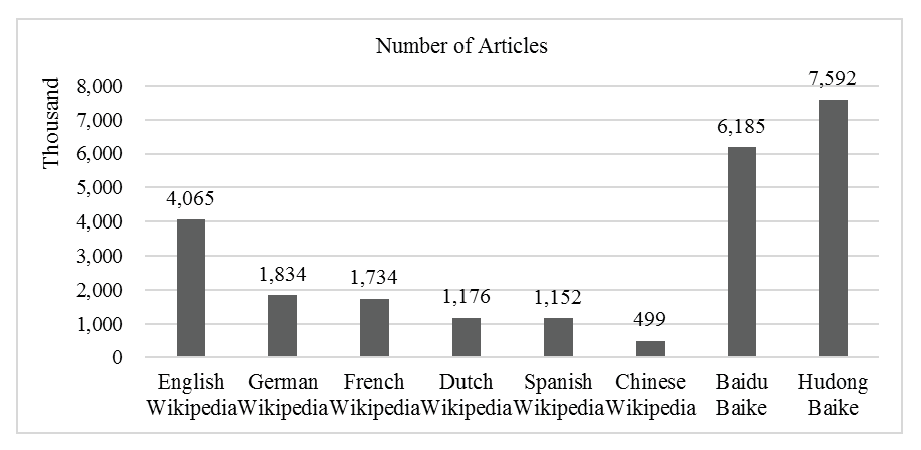
\includegraphics[width=0.8\columnwidth]{fig_stat}
  \caption{几个主要百科词条数量分布情况}
  \label{fig:wiki-stat}
\end{figure}

事实上,国内存在一些知名的通用领域的商业化百科全书,如百度百科\footnote{http://baike.baidu.com/}与互动百科\footnote{http://www.baike.com/},这些在线百科经过数以万计的人员撰写修改,已经形成很大规模,并存有丰富的中文知识。其中百度百科作为目前中国最大的开放式网络百科全书,收录了许多特色词条,因为参与编辑的人数多,编辑方式相对自由等原因,信息也更为全面。截止到2016年1月已收录词条超过1,313万条,远超过维基百科的中文词条数量。互动百科也有1430万个词条。如果能融合两个中文百科的信息,平衡中英文知识量级就可能实现。

国内切实存在一些商业化的中文知识库,如搜狗“知立方”和百度“知心”,它们都是以人性化搜索、个性化推荐为出发点所建立的知识图谱产品。研究领域也有Zhishi.me\cite{niu2011zhishi} 等中文知识库。然而,随着开放链接的增多,人们发现单语言数据集已经不能满足语义万维网知识融合,知识共享的特点。除了更好的融合多语言知识,跨语言链接还用来辅助机器翻译\cite{niehues2011using}、跨语言信息检索\cite{giang2015building}等。然而因为维基中文知识匮乏,中英文难以对齐等原因,中英文的跨语言链接还很少。

为解决中文知识匮乏问题,我们构建的大规模跨语言知识图谱XLore,充分利用最大的中、英文异构在线百科丰富的信息,即结合了中英文维基、百度百科、互动百科的知识,将词条、分类与信息框分别抽象成知识库中的实例、概念、属性,并利用维基的语言链接信息与跨语言链接扩展方法\cite{wang2012cross},添加双语知识的\textit{SameAs}关系,成功将双语语义信息融合在一起,为中英文知识共享打下了基础。

\section{挑战}

虽然目前知识图谱的构建已经有大量实践成果,我们的跨语言知识库XLore也在提供了一定中英文对齐知识,但知识库的完善,跨语言知识的增多,依然存在很多问题亟待解决。

本体作为知识库的骨架,其准确性与完整性非常重要。通常本体包含概念与属性,概念是对一些相似事物抽象出的类别,属性对事物特性进行描述。在RDF的定义中,有一些已定义的核心属性,如Rdf:type建立了实例与概念的instanceOf关系,也可以自定义属性。DBpedia有7000多个自定义属性,以\textit{http://nl.dbpedia.org/property}的形式定义。

基于百科构建的知识库,通常会通过词条信息框补充属性。信息框是一个词条的脸面,它包含了该词条的基本的、重要的信息,读者通过阅读信息框,就可以了解关于词条大部分重要内容。信息框中的属性是对相应实体的特性的描述,可以认为它是实例的自有属性,由此为本体设立的自定义属性可达上万个。哪些属性可描述同一类实体?同一表达形式的属性是否表达着唯一含义?概念下与属性要如何准确地描述本体?这些问题的解决,对构建一个准确、可用的知识库,起着重要作用。

在跨语言知识库构建过程中,本体对齐是核心关注点。维基百科提供了跨语言的词条链接,大部分跨语言知识库,如DBpedia、YAGO,都利用此链接集合匹配中英文实例与概念。但是,维基百科没有直接提供属性跨语言信息,并且其公开的数据文件中,也不含有可用信息框属性对齐关系。基于信息框的自定义属性链接的缺失,使得基于百科的跨语言本体在属性阶层无法匹配,知识库骨架无法形成。

据最新统计,截止到2016年2月,英文维基带有信息框的词条数量约是中文维基9倍,中文维基带有信息库的词条数量约为总词条数量的1/4。当前如果仅仅依靠维基百科获得属性对齐关系,必然会受到维基中英文知识数量不平衡的局限。

如何获取更多的属性跨语言链接?引入其他数据源进行补充依然是可行方法之一。然而因为异构百科在属性表示方面的迥异,编辑规则不一致,从标签文本角度出发是很片面的,即使在同语言情况下,也有很多相同属性不能直接对齐。比如中文维基使用\textit{制片商},百度百科使用\textit{出品公司}作为电影制作公司属性的标签,中文维基常有\textit{旁白}、\textit{配乐作品}等百度百科不使用的属性,等等。充分利用多源信息对知识的查漏补缺、错误修正有很大贡献,但面临的问题也有所增多。

此外,异构百科对于属性的领域界限划分模糊不清,维基百科中,信息库模板很好的给定了描述一类实体的属性集合。其他百科如百度百科,不包含模板信息。面对无规则无限制的杂乱属性集,如何准确定义概念属性,制定受认可的、特定领域下的模板,从而更好的为属性对齐服务,是我们需要考虑的难题。

属性的分析,对准确地描述本体、构建知识库起着重要作用。据我们所知,当前还没有中英文知识库对属性有过全面的分析与处理。XLore中虽然含有来自四个百科数据源的约6万个属性,但并没有进行进一步的跨语言对齐处理。如何处理异构百科的跨语言属性对齐,以及其衍生的一系列问题,从而完善我们的知识库,是当前亟需解决的问题。

基于知识库中属性的重要性,本文工作对百科的信息框属性进行了概念定义、同一查找、跨语言对齐等研究,力求获得更准确的本体框架,以及发现更多的跨语言链接。

\section{主要工作}
本节对文章涉及的主要工作进行初步的描述:从准确构建基于百科的知识库本体的目标出发,提出概念属性,在百科内尝试解决概念属性的生成、跨语言对齐等问题,以扶助构建跨语言本体,提高中英文信息的融合度。另外从知识库应用的角度出发,搭建展示系统与实体接口。本节根据之前提出的挑战,对涉及到的研究点进行了概括。

\subsection{维基百科概念属性生成}
针对本体中概念下的属性集合问题,我们定义概念属性,来表征某概念下一类实体的特性。维基百科中具备的信息框模板,对特定领域内实体的描述进行了规范,囊括领域范围内的属性集合。通过分析信息框模板,可以获得一系列概念属性。我们获取了维基百科大部分概念属性,该结果可覆盖维基中90\%以上的词条的信息框,为后续对概念属性的进一步研究打下了良好基础。

{\heiti 问题定义:} 给定一种语言的维基百科$W$,通过分析模板$T$,取得一系列概念$C$,以及相关的概念属性$\Rho_C=\{P{c_i}|i=1,2,...j\}$。

\subsection{异构百科跨语言属性对齐}
不同于大多数的跨语言属性对齐研究,本文将属性定义为概念属性,并同时进行百科异构性的分析,即对属性的研究建立在维基百科与百度百科两个异构百科上。结构与语言的双重障碍,为属性对齐的研究增加了难度。为尽可能达到结构上的统一,我们对无模板的百度百科属性集合生成概念属性,形成领域下的模板,并将属性对齐问题限定在概念领域范围下,同时利用中文维基为英文维基与百度百科搭桥引线,获取更多关联信息。

总结来说,本问题通过四个步骤解决并优化,分别为:1)生成百科概念属性模板,2)同语言对齐与相似属性合并,3)跨语言种子集合生成,4)跨语言属性对齐。

{\heiti 问题定义:} 给定两个中英文异构百科$W_{e}$与$W_{z}$,在限定领域$C$下,获得该属性集合,生成领域模板${T_{C}}$,并在该模板下,聚集相似属性组成超级属性$sp$,对齐跨语言属性$sp_{e} \Leftrightarrow sp_{z}$。

\subsection{中英文跨语言知识库的构建与应用}
本文提及的知识库系统XLore,其构建初衷是为解决中文知识匮乏问题,提高知识融合度与共享率,面对当前多语言在线百科与知识库中中英文信息极度不平衡的现状,利用其他丰富的中文资源不失为一则良策。基于此我们将目光聚焦在国内信息最丰富的两大在线百科全书——百度百科与互动百科上,利用两大百科的词条页面信息、分类体系数据,并结合维基百科对外发布的数据存储文件,抽取结构化信息,经过一系列的知识处理流程,获得语义信息,构成跨语言知识库XLore。图\ref{fig:xlore-procedure}为XLore的构建流程。

\begin{figure}[H]
  \centering
  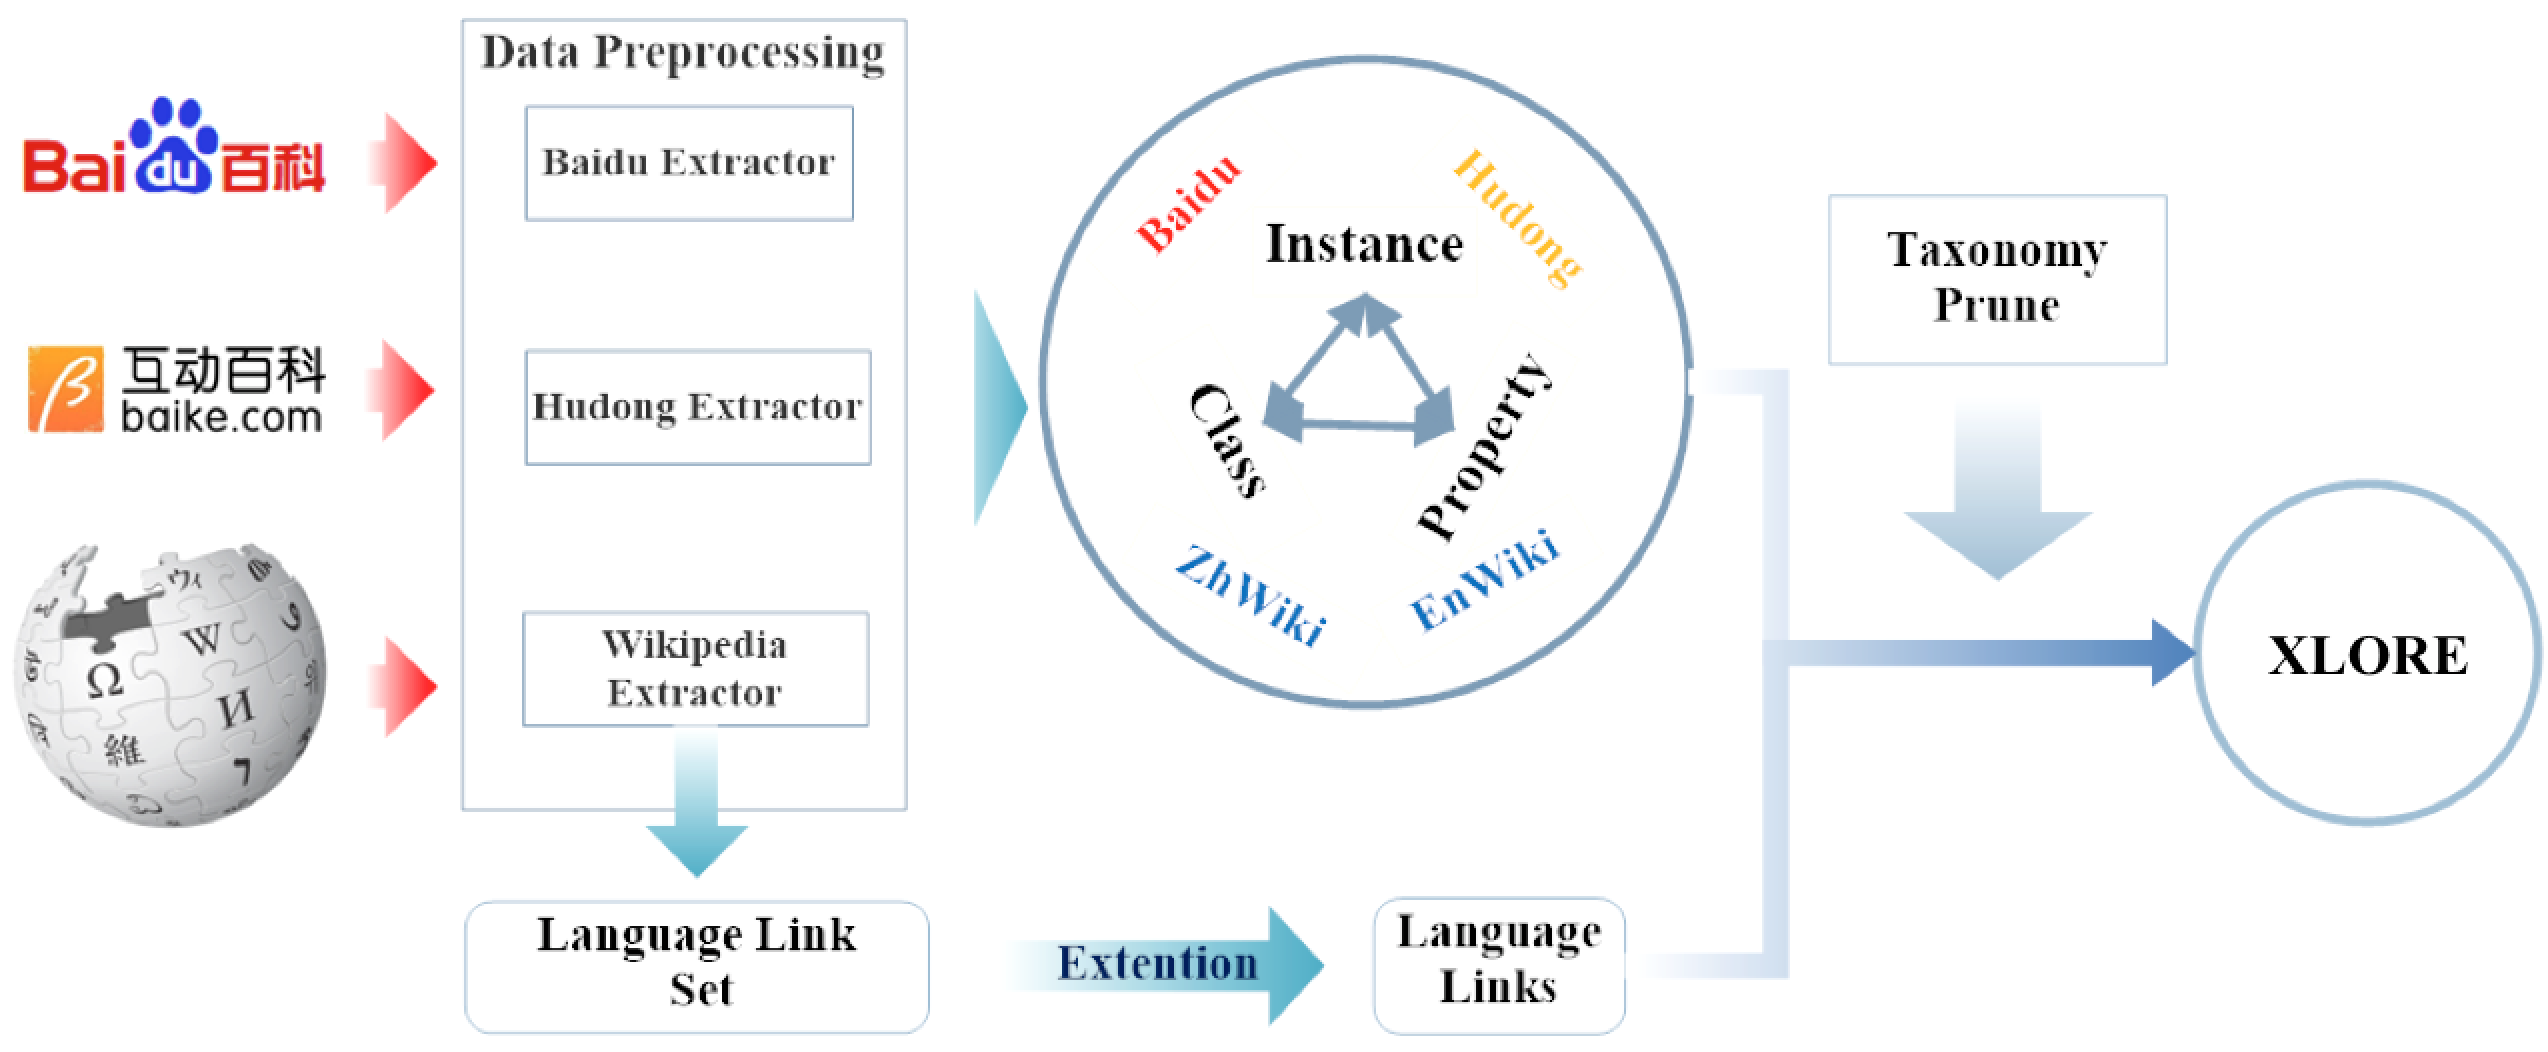
\includegraphics[width=0.8\columnwidth]{xlore-procedure}
  \caption{知识图谱XLore构建流程}
  \label{fig:xlore-procedure}
\end{figure}

值得一提的是,我们对XLore知识库的应用层次上也进行了尝试,主要体现在支持数据访问的在线系统XLore.org,以及提供实体语义信息的API接口,该接口支持限定领域查询与通用领域实体查询。

\subsection{主要贡献}
本文提出了一种概念属性生成与领域跨语言属性对齐的方法,并利用对齐结果与四个百科数据源的抽取结果,构建通用领域的中英文知识库XLore,其中主要贡献列举如下:
\begin{enumerate}[1)]
\item {\heiti 概念属性的定义与生成,} 工程抽取与算法计算相结合,提取出英文维基百科与百度百科两个异构百科下的信息框属性关系。包括百科下属性模板生成,与限定领域下的中英文属性匹配。该方法在构建大规模知识库过程中,对于从多语言的异构数据源生成对齐的shema有一定的贡献。
\item {\heiti 异构百科下的跨语言概念属性对齐,} 工程抽取与算法计算相结合,提取出英文维基百科与百度百科两个异构百科下的信息框属性关系。包括百科下属性模板生成,与限定领域下的中英文属性匹配。该方法在构建大规模知识库过程中,对于从多语言的异构数据源生成对齐的shema有一定的贡献。
\item {\heiti 构建跨语言知识库XLore,并提供多元化的数据展示与应用接口,}前者分别从一般用户与专业用户的不同角度,给出搜索框查询与SPARQL查询两种知识访问方式;后者考虑知识库的应用场景,提供基于RestFul的实体访问API,对给定文本进行实体分析与排歧,返回实体语义信息,实现了一定应用价值。
\end{enumerate}

\section{论文组织}

本文通过绪论、研究现状、基于维基百科概念属性生成、基于异构百科的跨语言属性对齐、中英文知识库XLore系统与应用接口、总结与展望共6个章节来组织全文内容,其章节关系与结构组织如图\ref{fig:organization}所示:

\begin{figure}[H] % use float package if you want it here
  \centering
  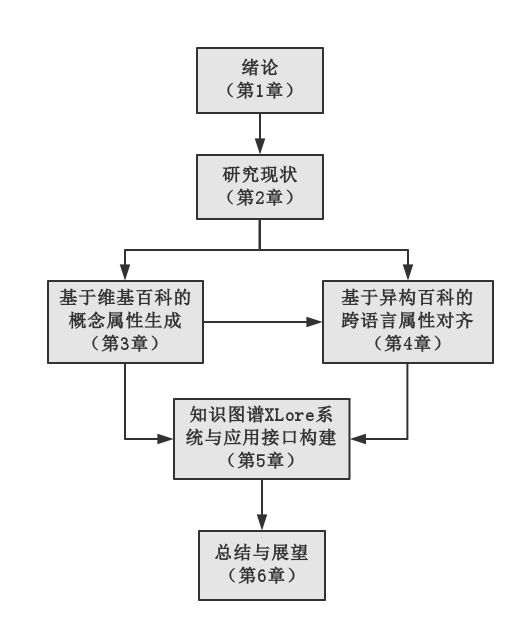
\includegraphics[width=0.5\columnwidth]{organization}
  \caption{论文组织结构图}
  \label{fig:organization}
\end{figure}

第 1 章为绪论,对本文的研究背景进行描述,提出可能的挑战,并概要地介绍工作内容,交待论文的主要贡献及文章组织结构;

第 2 章为研究现状,介绍当前构建的跨语言知识图谱的发展情况,列举当前广为人知的多语言与中文单语言知识图谱,并介绍其构建技术;并对跨语言本体对齐研究现状进行描述,包括schema对齐,属性对齐等;此外从知识库应用角度,介绍实体链接的常见研究点。

第 3 章详细分析了维基百科的信息框编辑规则,对数据文件中的模板给出了分类与处理方法,由此定义概念属性,并以覆盖大部分词条描述为目标,借由模板生成概念属性;

第 4 章说明了基于异构百科的跨语言属性对齐流程。首先通过观察与抽取百科中的模板与属性,提出异构百科属性研究的种种难点,之后为百科属性集合提取概念属性模板,并实现在特定领域下,同语言相似属性的对齐与跨语言属性链接;

第 5 章简要介绍了基于多源异构在线百科,构建跨语言知识图谱XLore的过程,重点展示了为XLore搭建的可视化系统与数据访问接口,从实际应用角度展示该知识图谱的结构化与可用性;

第 6 章对本文提出的跨语言属性对齐与知识图谱构造研究工作进行了总结和展望,分析了不足之处,为下一步研究提出了新的建议和意见。
 
%\subsection{页面元素介绍}
%
%四个在线百科的词条页面在布局上很相近。通常,一个词条页面可以贡献两种带有潜在语义信息的元素,分别为所属分类信息与词条内容信息。分类信息包含负分类、自分类及其上下位关系信息。 图xxx是互动百科分类页面的截图。
%
%一个词条页面描述了一个显示中的实例。这些实例的丰富的信息由一个或多个经过专业认证的编写者们创建或修改,一般其信息内容都一定的可考证依据。另外,一篇词条可能归属于一个或多个分类。词条自带的实例内容、其与其他词条的关系,以及它所属的类别,都在构建知识库时起着重要作用。一般来说,一篇词条页面中,有五种元素可以被利用:
%
%{\heiti 标题:} 词条标题,即其所表征实体的名称,可以作为区分不同实体的表识,其内容在同一百科中是唯一、不可重复的。维基百科、互动百科、百度百科都对重名的不同实体做消歧处理,并在标题上表现出来,比如。。。
%
%{\heiti 摘要:}摘要是实体的一端剪短的简介,通常包含该实体的重要信息。一般是页面正文的第一段话。
%
%{\heiti 信息框:}一部分词条中带有信息框。信息框是一个表格形式,内含属性-属性值对,带有实体重要的属性信息。从信息框中可抽取主语-属性-属性值的三元组格式的结构化信息,其中主语即为该词条所表征的实体。
%
%{\heiti 链接:}词条文本中的超链接部分,是另一个词条的入口,点击即可进入对应词条的页面。它表征该词条与百科中其他词条的关系,是构成知识库中实体与实体关系的重要信息。
%分类:一个词条所属分类一般在该词条页面的底部一行显示,已标签或超链接的形式渲染。一个词条可能归属于一个或多个分类,表征知识库中的is-a关系。
%
%图XX是一篇中文维基的词条页面
%
%需要提到的一点:维基百科中页面内容的组织是遵从于维基模版制成的。此模版对词条编辑时,所要遵循的内容、结构等信息进行了约束。比如xxx,xxx。信息框的填充也从模板中产生。比如:词条 星际穿越根据模板Infobox film来编写,按规定来说,电影词条的信息框信息都应根据此模版来编辑。信息框模板带有电影领域公认的、常用的属性集合。
%
%除此之外,维基百科中,大部分词条的页面左边栏中,还提供了跨语言链接,该链接指向其他语言下该实体的词条页面。利用这些人工构建的跨语言信息,我们可以获得初步的跨语言链接集合。
%

\chapter{研究现状}
\label{cha:research}
本章对知识库的发展现状与构建相关技术进行了研究与探讨,详细介绍了DBpedia等知名知识库,并对跨语言本体对齐技术进行了梳理总结。在这些研究的启发下,结合实际问题与切实数据情况,提出Schema层中概念属性对齐方法。此外,对知识库应用的一个重要分支—实体链接技术进行了调研。

\section{本章引论}
%自从Time Berner-Lee提出语义万维网的概念并规划出发展前景,语义网逐渐受到研究领域的关注,开始快速发展。通过语义万维网的直接目标:即让计算机理解语义文本,加强自动交流,可以预见语义网的建立要结合人工智能与Web技术。以自然语言处理、信息检索、机器学习为首的人工智能负责对纯文本进行分析、清理、语义理解、知识融合等工作,而Web技术则主导解析HTML文本,以及为知识关联与利用提供语义化环境等。从当前技术的发展趋势来看,作为人工智能与Web相结合的产物,语义网的出现,也是万维网发展的必然结果。

知识图谱作为语义网发展过程中的产物,最初由谷歌提出,是谷歌对其建立的知识库产品的称呼,现在这一名称被广泛用来指代大规模知识库。知识图谱涵盖大量实体,包括实例、概念、属性三类主要元素,以三元组的形式,即“主语-谓语-宾语”,表示关系。一般来说,一个实例属于一个或多个概念,并含有多个属性与属性值,即关系事实,表征该实例的特性。知识图谱规模庞大,一般从多个数据源中精炼而成,具有一定的容错性。多源知识的自动融合和关系抽取,一直是知识图谱领域广受关注的研究点。本章对知识库研究现状进行讨论,列举比较典型的知识库,探讨其优缺点(详见\ref{sec:knowledgebase-research}节),并应用角度,介绍实体链接常见问题与应用(详见\ref{sec:entity-research}节)。

基于海量数据分析构建知识图谱的一项重要任务为,即获取关系事实\cite{suchanek2014knowledge}。关系事实表征着实例的属性及实例间的关系,如“清华大学—建校时间—1911 年”、“清华大学—现任校长—邱勇”,均为关系事实。规模较小的领域本体,因实体类型限制在一定领域,所涉及的属性也屈指可数(成语感觉怪怪的),一般可以通过人工直接定义\cite{boyce2007developing}或人工抽取\cite{wang:movie}来获得。然而以百科等大型数据集为来源的知识图谱,通常从页面信息框中提取关系事实与属性,数量在万级以上,杂质较多,准确度不能保证。因此,基于百科分类树与信息框属性构建的知识库本体需要进行检测、清理、对齐等处理。\ref{sec:ontology-research}节中将会从本体对齐、跨语言属性对齐等方面来阐述近些年对本体或信息框属性的研究,这些工作与知识库构建息息相关(同怪怪的),对我们的概念属性工作有着很大的指导意义。

\section{知识库构建和相关技术}
\label{sec:knowledgebase-research}

随着语义网概念的普及与技术的发展,不同领域、不同规模的知识库层出不穷。发布在LOD上的知识库林林总总,既有DBpedia、Freebase、Wikidata等著名的大型多语言知识库,也有限定领域的LinkedMDB\cite{erxleben2014introducing}、GeoNames\cite{wick2011geonames}等。这些知识库为实现全球知识共享的远景做着不懈的努力。

除此之外,一些知名公司也在做着相关产品,比如知识图谱的领头羊——谷歌的Google Knowledge Graph\cite{singhal2012introducing},以及微软研究院的EntityCube\cite{nie2012statistical}和Probase\cite{wu2012probase}、IBM的Watson项目\cite{ferrucci2012introduction}。国内也涌现了一批商业化的中文知识库,如搜狗“知立方”和百度“知心”。商业领域对知识图谱的期望,主要在于优化搜索。与传统搜索相比,基于知识图谱的搜索在两方面有所改变:1)从搜索字符串入手,对查询内容进行了语义上的分析,从而精准地理解用户意图,实现更为人性化的搜索;2)在返回结果方面,知识图谱可精确返回确切的实体或文本,并可额外提供系统的结构化相关信息,Search Engine Land称谷歌利用知识图谱,提供的是答案,而不仅仅是一堆链接\cite{sullivan2012google}。

随着知识图谱知识关联、可推理等特点逐渐浮出水面,其用武之地已经不局限于搜索引擎,个性化推荐也成为企业建立知识图谱产品的出发点\cite{Burke00knowledge-basedrecommender,aggarwal2016knowledge}。利用知识图谱的信息关联,能很容易地找出相似或相关实体,很好地解决了基于评分推荐所面临的冷启动问题。文献\cite{passant2010dbrec,kaminskas2012knowledge}基于DBpedia建立音乐知识库,从地方兴趣的角度推荐音乐。除了产品推荐,实体推荐知识图谱的一项重要应用。Yahoo!开发了名为Spark的实体推荐引擎\cite{blanco2013entity},旨在用户搜索时,提供相关的其他实体,如搜索演员时推荐有合作关系的作品与合作人,类似的功能在谷歌搜索与百度搜索上也可看到。此外,有不少企业利用知识图谱的语义关系,实现社交网络上的好友推荐\cite{venkataramani2012tao},信贷领域的借贷人识别\footnote{\url{http://www.slideshare.net/sfbiganalytics/bigdata-and-ai-in-p2-p-industry-knowledge-graph-and-inference}},以及知识图谱支持的自动问答等\cite{yih2015semantic,yang2014joint}。

知识图谱的建立涉及很多挑战,包括知识抽取、多源知识融合、知识的推理与应用等。其中多源知识融合是比较困难的一个环节,因为不同数据源的数据构造规则不统一、人工编辑用语习惯不一致等问题,使得知识融合不能单纯合并,需要识别不同源中同一实体、同一属性,找到对齐关系,构建统一的本体。整个过程,需要自然语言处理、机器学习等诸多关键技术的辅助。

下面通过描述几个知名知识库的构建方法,介绍知识库构建思路,这对我们构建跨语言知识图谱有很重要的参考意义。

\subsection{中文知识库}

Zhishi.me\cite{niu2011zhishi,wang2014publishing}是国内学术领域最早构造的中文知识库,它从三个大型中文在线百科,即中文维基、百度百科、互动百科中获取知识,共抽取了500万个不同实体,包含百科中的摘要、超链接、分类等诸多信息,组成RDF三元组。因为融合多个百科资源,Zhishi.me运用了匹配算法跨百科寻找$\langle owl:sameAs\rangle$ 关系,主要通过词条标题处理实体对齐,用重定向信息解决歧义问题。最后,Zhishi.me利用维基百科现有跨语言链接对齐到DBpedia,从而与LOD数据集关联。

另一个中文知识库CKB\cite{wang2011building}基于互动百科构建。该知识库首先从百科自带分类体系和信息框中定义并抽取出概念层次结构以及属性,构成知识库本体架构,然后用本体描述百科中的每个实例,共生成了520万RDF三元组,包含19542个概念、2079个对象类型属性、302个数据类型属性以及802593个实例。最后,CKB同样利用维基百科的跨语言链接与DBpedia的实例相关联。建立在独立百科上的CKB并没有面临实体对齐等复杂工作,其构建思想是从本体出发,先给出明确、清晰的本体定义,再将实例挂到本体下,与规模较小的专业领域本体构建有异曲同工之处,但过程自动化。此外,CKB着重关注数据质量,对互动百科的原有分类体系进行了去重、去环等操作,相对于Zhishi.me,工作更细致,内容更准确。

我们的跨语言知识库XLore借鉴了Zhishi.me与CKB的构造理念,其构造流程在\ref{sec5:cross-lingual-knowledge-base}中给出介绍。

\subsection{多语言知识库}
DBpedia作为跨语言知识库的代表,最初版本在2007年发布\cite{auer2007dbpedia},是一个完全基于维基百科数据构建的多语言、跨领域知识库,注重于对实体、摘要等的提取,包含13个语言,共195万实体。之后DBpedia加强了对信息框的处理,提出DBpedia映射\footnote{\url{http://mappings.dbpedia.org/index.php/Main_Page}}解决信息框模板中属性一义多词的问题。目前DBpedia已经涵盖97个语言的知识,24.5亿个RDF三元组,成为LOD的核心。已有多个外部数据库或资料集与其相连,包括GeoNames、DBLP、Musicbrainz等。除此之外,DBpedia也作为诸多应用的基础数据支持,包括TAC-KBP\cite{mendes2011evaluating}的实体链接任务、音乐推荐\cite{passant2010dbrec}等。

%鉴于维基百科在信息框以及模板上的定义多元化,这一改善映对语言的机制,多是经过人工参与的。首先定义一个本体schema,再将维基信息框属性映射上去\cite{mendes2012dbpedia}。

%\subsection{多语言知识库YAGO}
另一个著名的多语言知识库YAGO同样创建于2007年,9年间已经更新三代。从最初的YAGO\cite{suchanek2007yago,suchanek2008yago},到关系事实扩展的YAGO2\cite{hoffart2013yago2},再到以多语言为特色的YAGO3\cite{mahdisoltani2014yago3},其更新历程也是知识库的发展趋势的一个缩影。
\begin{itemize}
  \item {\heiti YAGO}首次将WordNet\cite{fellbaum1998wordnet}与Wikipedia结合。其数据模型完全基于RDF标准,模型设计中详尽地描述与探讨了一对多关系、语义关系定义等问题,对其他知识库的建立有着很好的借鉴意义。在构建分类体系时,添加类型排查算法,保证YAGO的准确率达到95\%。YAGO含有约170万个实体,与1500万个关系事实。
  \item {\heiti YAGO2}是YAGO的扩展版本,在原版本基础上整合了更多的空间与时间维度的关系事实,并融合了GeoNames知识库信息,知识数量扩展到980万个实体,44700万个关系事实。
  \item 以往的YAGO版本都是纯英文知识库,{\heiti YAGO3}开始向多语言转换。YAGO3基于维基百科,扩充了德语、法语等10种语言,在跨语言对齐方面提出了简单却有效的方法,主要处理了关系事实与概念分类。前者从各语言信息框中抽取属性—属性值关系,经过类型判断与功能冲突判断后对齐属性;后者利用Wikidata中现有的跨语言关系,对齐数量受到Wikidata存储量的局限。
\end{itemize}

\section{本体对齐相关研究}
\label{sec:ontology-research}

本体是一个领域的术语集合,是对领域的描述,是知识库的“骨架”。多个本体或知识库要合并时往往会出现{\heiti 语义异构}现象,即不同本体对于同一概念的表达有偏差,直接合并不可行。本体对齐就是致力于解决语义异构问题的研究。另外,本体的表示也不仅仅局限于一种语言上,当涉及多种语言下的本体融合时,还需要解决跨语言本体对齐问题。本节从同语言的异构本体对齐、跨语言本体对齐方面分类总结,重点介绍信息框属性的相关研究。

\subsection{异构本体对齐}
常见的本体匹配方法可以归纳为:

{\heiti 基于文本的方法},即比较两个词语的相似度。字符串相似度对比是比较常见的方法,其中,编辑距离、N-gram距离等较为常用。此外也有通过语义信息来计算的方法,WordNet\cite{miller1995wordnet}在该方法中被广泛应用。

{\heiti 基于结构的方法\cite{hu2008matching}},即利用本体构成的图关系来进行比较。较为简单的方法是利用本体自带的限制信息,如定义域或值域的相关程度。另外也有利用本体关系进行相似度传播的算法,该方法需要一批已经匹配的种子集合,根据\textit{临近实体也可能很相似}的假设,寻找更多匹配对。

{\heiti 基于领域知识库的方法\cite{ponzetto2009large,gligorov2007using}},领域知识库为实体提供了背景信息,并认为背景相似的实体可能匹配。

{\heiti 基于机器学习的方法\cite{niepert2010probabilistic,albagli2012markov}},即将匹配问题抽象为分类或优化问题,引入分类算法、概率模型等机器学习方法解决问题。

%当前已经得益于OAEI(Ontology Alignment Evaluation Initiative)比赛

\subsection{跨语言本体对齐}
当前跨语言本体对齐可以分为5类\cite{},分别为:

{\heiti 人工处理\cite{}:},即直接手工对齐;

{\heiti 基于语料对齐:} 文献\cite{}中用此类方法对齐英文WordNet与中文HowNet;

{\heiti 基于实例对齐:} 即通过实例相似度做对应关系的计算\cite{};

{\heiti 基于语言对齐:} 将丰富的语法语义分析结果作为本体特征,便于对齐。

{\heiti 融合多方法的框架:} 文献\cite{}中提出的跨语言本体对齐框架,以及OAEI测试中的RiMOM系统\cite{},都是通过先翻译到目标语言,然后在单语言上运用结构对齐、词汇对齐等方法实现跨语言对齐。

\subsection{信息框属性对齐}
\label{sec:property-research}
属性是本体重要的组成部分,一般本体、尤其领域本体中定义的属性较少,通常通过人工检查对齐即可\cite{wang:movie},而通过在线百科构建的知识库,其中本体多从信息框中抽取生成,数量较多。当前已有大量针对信息框与属性的研究,主要包括属性抽取、相似属性查找、信息框填充、跨语言属性对齐等方向。

{\heiti 属性抽取}指从普通文本或结构化数据中抽取属性对工作,通常基于词法—句法规则匹配方法\cite{pacsca2007role,lee2013attribute},或从网页表格或列表中通过$\langle td\rangle$,$\langle li\rangle$等标签获得\cite{crestan2010web},并且通过不同的测量方法过滤掉错误结果,如基于出现频率\cite{pacsca2007role}、人工规则\cite{lee2013attribute}等。本文针对维基百科特点,给出基于信息框属性的抽取过程,将在\ref{sec:property-extraction}中详细说明。

{\heiti 相似属性查找}的目标是将表示相同意义的属性找出并合并。此工作可以转换成寻找相似字符串的问题,最简单的思想是利用字符串相似度匹配方法,常见的算法有余弦相似度算法、Jaccard距离算法、编辑距离等。
其他的衡量方法依赖已有的知识资源(如WordNet)\cite{yang2005measuring},或者语境分布\cite{pantel2009web}。
大部分寻找同义属性的工作都是基于英文的,中文相关工作较少。并且,由于中文方块字特征(如没有大小写区分、没有空格等),基于中文属性的工作则更加困难。文献\cite{liu2014extracting}以百度百科为数据源,结合文本相似度、语义相似度、上下文相似度,寻找中文相似属性。

{\heiti 信息框填充}可以看作是信息抽取问题,从词条文本中抽取主语-关系-宾语三元组,为缺失属性抽取属性值。KYLIN\cite{wu2007autonomously}是第一个解决信息框缺失问题的系统,它使用自监督方法,在训练数据足够时效果不错。WikiCiKE\cite{wang2013transfer}在跨语言数据集上,使用基于迁移学习的方法,利用英文丰富的知识填充中文信息框。

{\heiti 跨语言属性对齐}旨在匹配不同语言下对应信息框中的属性。当前常见方法为在维基百科已知的对齐词条下,通过对属性值的比较,对齐同一属性。其中基于字母系统的语言比较起来相对容易,可以直接利用字符串相似度计算等方法\cite{bouma2009cross}。而英语与方块字的对齐往往要经过翻译工具辅助\cite{fu2009cross},文献\cite{nguyen2011multilingual}则利用。

判定对齐分为非监督方法与监督方法,前者通过数据特性,在标签文本、链接结构、共现性、值域范围等方面指定相似计算方法与基准,保留可能性大的匹配对\cite{nguyen2011multilingual,lin2011unsupervised};后者将问题抽象成是否匹配的二分类问题\cite{adar2009information},通过设定特征集合训练模型获得准确结果。另外因为受到已对齐词条的局限,也有先找到更多跨语言词条,进而增加对齐属性数量的方法\cite{rinser2013cross},或者通过已对齐属性扩展对齐词条,进而迭代处理属性的方法\cite{nguyen2013slint}。

维基百科的模板特性影响着人们对于属性的定义,属性对齐过程中,应该在何种粒度上操作?大部分研究认为标签相同则为同一属性\cite{adar2009information,nguyen2011multilingual},也有将不同模板下的属性区分开来\cite{bouma2009cross}。本文认为不同概念下的属性表征含义不同,通过模板抽象出概念区分属性。

\section{实体相关技术}
\label{sec:entity-research}

知识库的一个重要应用是实体链接(Entity Linking),即将文本中出现的命名实体文本链接到知识库中对应实体上。实体链接是链接网络文本数据与知识库的桥梁,在很多不同领域中有所应用,比如信息抽取\cite{lin2012entity,nakashole2012patty}、文本分析\cite{gattani2013entity}、问答系统\cite{gattani2013entity,welty2012comparison}等等。TAC(Text Analysis Conference)将实体链接作为Knowledge Base Population(KBP)的一个子任务,并提供数据集供参赛者评测。

实体链接需要解决三个主要的子任务,即实体候选生成、实体候选排序、未链接文本预测。下文从任务描述与常用解决思路方面对它们进行简单介绍。

{\heiti 实体候选生成}旨在建立一个名称与知识库实体的对应关系,实体链接的任务往往是首选在文本中识别出名称,再进一步分析可能对应的实体。因此实体候选是决定能否链接的关键步骤。通常情况下,实体候选集合从百科数据中抽取\cite{bunescu2006using,shen2012linden,shen2013linking},维基百科中的词条标题、重定向页面、消歧页面、超链接等,都可以作为实体名称。此外也有一些扩展方法,比如基于规则匹配\cite{han2009nlpr_kbp,lehmann2010lcc},取公司首字母缩写、人名缩写等,有监督学习的方法\cite{zhang2011entity} 以及利用搜索引擎查询字符串扩展候选集的方法\cite{dredze2010entity, monahan2011cross}。

{\heiti 实体候选排序}是实体链接任务的关键步骤,给定一个表示文体,如果它对应多个实体,需要用排序算法进行消歧,确定最匹配实体。目前提出的排序模型主要分为监督排序方法与非监督排序方法。前者通过对训练数据集进行学习,预测给定候选是否是指定实体,包括二分类方法\cite{zhang2010entity,lehmann2010lcc,monahan2011cross,chen2011collaborative}、概率方法\cite{han2011generative}、基于图的方法\cite{han2011collective}。后者不需要预先标注的数据,方法包括向量空间模型\cite{cucerzan2007large,han2009nlpr_kbp},基于信息抽取的模型\cite{varma2009iiit,gottipati2011linking}等。

{\heiti 无链接文本预测}是指:给定一个实体名称,知识库中没有对应实体的问题,这是基于候选集合所必然出现的局限。一些研究默认实体候选包含了所有可能的实体名称,从而忽略了这个文本\cite{cucerzan2007large,kulkarni2009collective,shen2012liege},或者返回NIL\cite{varma2009iiit}。有的系统对于返回实体进行了更为慎重的筛选,即设定一个阈值,如果实体的可能性小于这个阈值,那即便它是最佳候选,也不认为它是所求实体\cite{han2009nlpr_kbp,lehmann2010lcc,han2011generative}。

本文为跨语言知识库XLore开发了实体链接API,旨在为给定文本或实体提供相关语义信息,实现XLore可应用目标,在实践中完善知识库。

\section{本文研究目标和思路}
本文总体目标为应用信息抽取、机器学习等方法,对跨语言异构百科信息框属性进行概念属性生成与对齐,并将结果应用到跨语言知识图谱构建上。重点对中英文维基生成概念属性,针对英文维基与百度百科的异构性提出属性对齐流程与框架,致力于获得更多信息框属性。在构建知识库过程中使用属性对齐结果丰富知识链接。最后为观察知识可用性,实现知识应用,开发展示系统与实体链接接口,以支持数据访问。下文将给出本文工作的主要思想与方法描述。

\subsection{基于维基百科的概念属性生成}
属性作为知识库Schema中的重要元素,与概念有着密切关系,用来描述概念下的实例特性,而不同概念的性质不尽相同。我们将指定概念下的实例特征定义为概念属性,并认为属性的歧义性(相同名称的属性,可能指代不同的意思)受限于其概念领域,如名称为\textit{产地}的属性,在电影领域中是\textit{制作国家}的意思,而在植物领域中是\textit{生长地点}的意思。概念属性可以对属性进行精确的区分。

维基百科通过{\heiti 信息框模板}规范着对同一领域的实体的描述规则,模板中的属性为一类实体的特性,与概念属性很相近。通过分析维基百科模板,利用模式匹配,我们获得了一系列概念,以及概念下的属性集合(详见第\ref{cha:concept-property}章)。

%在属性抽取一步,百度百科的网页结构化信息较为容易处理,但维基百科信息框所依据的模板,定义却不统一。通过对维基百科模板的观察,我们为不同的模板定义提供了相应的抽取规则,将可能获得维基百科信息框模板与属性数量最大化(详见\ref{sec:property-extraction})。

\subsection{基于异构百科的跨语言属性对齐}
大部分对跨语言属性对齐的研究都在维基百科上进行,
%维基百科丰富的知识储备、多语言的特性,有利于研究者探寻数据规律与特征。
然而,中英文维基知识相差悬殊,无论是词条还是信息框,数量都不对称。要想尽可能多地获得中文属性与跨语言关系,我们需要其他中文百科的辅助。

本文的工作重点为异构百科上的跨语言属性链接。为解决引入多源数据所面临异构特性所带来的百科规则的不同、人员编辑习惯的迥异等问题,我们对维基百科与百度百科的模板与属性的异同进行了详细的分析(详见\ref{sec:template-property-analysis})。

我们提出跨语言属性对齐框架(详见\ref{sec:property-matching}),跨语言对齐被看作是一个二分类问题,为达到更精确的结果与更高的召回率,我们首先对齐同语言信息,为跨语言做好铺垫;抽取跨语言种子,避免人工标注。

我们依然引入概念属性,在没有模板的百度百科下圈定概念与属性集合,形成领域模板。此后,属性的分析在模板范围之内进行,减小了搜索空间,使算法运行效率有所提高(详见\ref{sec:domain-template})。

概念属性避免了一词多义,但属性还存在一义多词现象,即描述相同意义的属性,有不同的写法。比如电影\textit{上映时间}有\textit{首映时间}等多种写法,这种现象多是由于编辑者个人写作习惯不同所造成。找出同领域的这些同义词,有助于丰富链接知识。
%我们从文本相似度、语义相似度等方面出发,计算同领域的属性集合中的两两相似性,将相似性高的属性合并成同一个属性(详见\ref{sec:similar-property})
我们通过多策略对齐中文维基与百度百科,找到维基属性与百度属性的一对多关系,从而获得相似属性(详见\ref{sec:similar-property})。

得益于维基百科的多语言特性,通过模板对齐、属性值匹配等方法,可预先获得一批精准度高的属性跨语言对齐关系。但以中英文维基对齐属性为桥梁匹配的维基与百度百科属性,仅是一小部分,因为百科异构性,还有大量的中英文跨百科属性有待具体分析。这批初始的跨语言对齐属性,将作为进一步抽取更多属性对齐关系的种子集合。这一步更避免了监督学习问题常见的训练集合的标注问题(详见\ref{sec:cross-lingual-seed})。

以上几个模块在一定程度上削减了百科异构性带来的阻碍。相对于字母系统语言下的属性对齐研究,中文与英文在写法上大相径庭,不可单纯依赖文本相似度。本文将跨语言属性对齐看作二分类问题,除了使用文本特征,还提出几项假设,比如同一属性的使用流行度相似、同一属性的对象值指代同一个实体等,从结构维度抽取跨语言对的特征,辅助扩展跨语言链接的实现(详见\ref{sec:cross-lingual-property-matching})。

\subsection{XLore系统与应用接口构建}
本文以解决中文知识匮乏现象、提供中英文链接知识为出发点,构建跨语言知识库XLore。为了能直观地观察数据,我们为XLore搭建网页展示系统。提供开放式的数据访问,包括点击访问、搜索框查询、SPAQL语句查询、关系可视化等。从应用的角度,还搭建了基于知识库的实体链接查询接口,供文本相关研究调用(详见第\ref{cha:xlore}章)。
%基于当今知识库的构建思想,我们以维基百科、百度百科、互动百科为数据源,从异构结构中抽取实例、概念、属性构成知识库。跨语言链接是融合多语言知识库的根本要素,我们对三类元素的链接分别进行了扩展,丰富了跨语言关系。
%之后将结构化数据转换成RDF三元组,构成标准知识库

\section{本章小结}
本章首先从知识图谱的应用角度介绍了其重要性,梳理了涉及的问题与相关技术,包括中文及跨语言知识库构建、本体对齐、跨语言属性对齐以及实体链接技术。最后,总结了相关研究的优势和不足,并结合本文工作的特色,凝练了研究目标和问题,形成自己的问题解决思路,提出具体解决方案。
\chapter{基于维基百科的概念属性生成}
\label{cha:concept-property}

\section{本章引论}

知识库构建过程中,本体作为骨架,占有重要地位。本体对概念下的实例进行描述,包含一系列概念与属性,属性为概念下一类实例的共有特性。

为了获取通用领域下概念与属性的关系,本章中,我们对维基百科进行了详细地观察与解析,获得了维基中模板与属性的规则。

维基百科鼓励编辑者使用模板对词条以及信息框进行组织与编辑。模板是百科针对不同主题的词条内容所列出的标准结构框架,类似于长期积累形成的标准写作规范。模板使词条的结构变得有规律可循,也可以有效避免关键信息的缺失。信息框的编辑也可模板化,信息框模板包含了描述一类实例的常用属性。图\ref{fig:template-infobox-film}为\textit{Template:电影信息框(Template:Infobox Film)}\footnote{https://zh.wikipedia.org/wiki/Template:电影信息框},其中含有电影的诸多属性,如\textit{演员,导演,时长}等。模板在一定程度上描述了一个领域的信息,充分利用其中信息,对概念-属性关系的研究有很大意义。

本文主要对信息框属性进行研究,后文中提到的模板,同一指代{\heiti 信息框模板}。

\begin{figure}[H]
  \centering
  \fbox{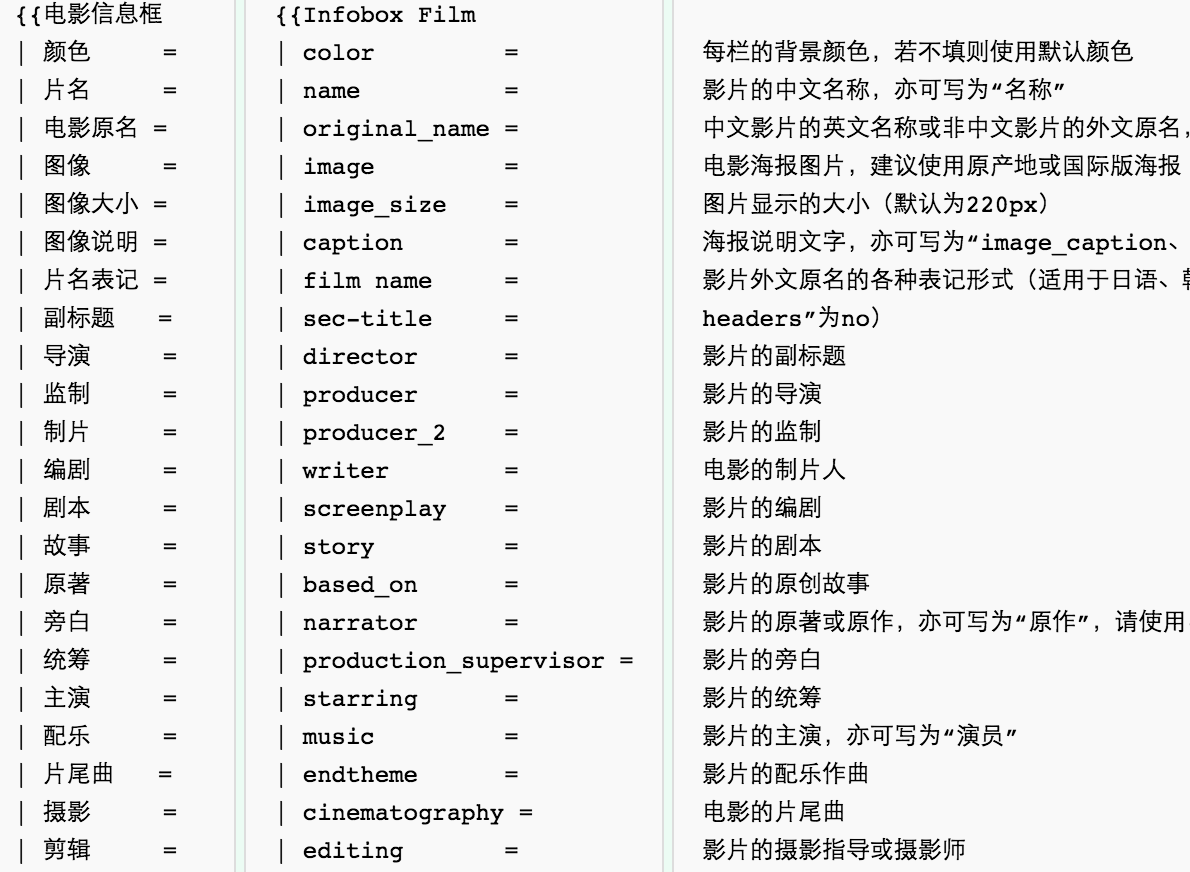
\includegraphics[width=0.8\columnwidth]{template-infobox-film}}
  \caption{电影信息框模板}
  \label{fig:template-infobox-film}
\end{figure}

基于对模板设计的思考,我们提出概念属性:即概念下有特定的属性集合对实例进行描述,属性的定义依赖于概念,不同概念下的属性意义可能不一样。以领域信息区分属性,有助于避免属性歧义问题。同时,考虑到维基信息框模板规范着一个概念下对实例的描述,我们可以用{\heiti 属性@模板}定义一个属性。

因为百科数据杂乱,概念属性生成的工作繁琐但至关重要,结果的数量与质量,在很大程度上影响着其他属性研究的准确率,过多杂质的引入会增加相关工作的难度。

本章工作充分利用维基百科的结构化信息,从中英文数据文件中,提取概念属性,其结果覆盖了90\%以上的维基词条,为今后对信息框属性的进一步分析打下了良好的基础。

\section{维基百科信息框模板与属性分析}
\label{sec:template-analysis}

维基百科自2001年创立,经过15年左右的发展,不仅储备了海量数据,在编辑规则上也越发规范。但因为词条繁杂、参与人数众多,还是无法保证数据统一,质量差强人意,这使生成概念属性的工作困难重重。

具体来说,维基所提供的数据文件\footnote{https://dumps.wikimedia.org}中,词条信息框的内容是以{\heiti 模板标签}来组织的,而模板标签与真正展示在网页上的{\heiti 显示标签}不同。模板标签与显示标签的关系在对应语言的信息框模板词条下有定义。图\ref{fig:film-tl-rl},电影\textit{疯狂动物城}的配乐为\textit{迈克尔·吉亚奇诺},这条信息在词条中的数据文件中是\textit{music=[[麥可·吉亞奇諾]]},而在网页中的显示是\textit{配乐作曲 \ 迈克尔·吉亚奇诺},其中,\textit{music}为模板标签,\textit{配乐作品}为显示标签,而两种标签的对应关系,在词条\textit{Template:电影信息框}中有所说明(见图\ref{fig:template-infobox-film})。维基百科的这种设计,使模板属性在不同语言上有了标准规范。对于任意一个语言,在设计自己的电影信息框模板时,只需根据模板标签,给出对应的显示标签即可,对多语言百科来说,不失为一种好方法。但是间接获得显示标签,也对模板的获取增加了难度,而人为设计的不规范性,又雪上加霜。

\begin{figure}[ht]
  \centering
  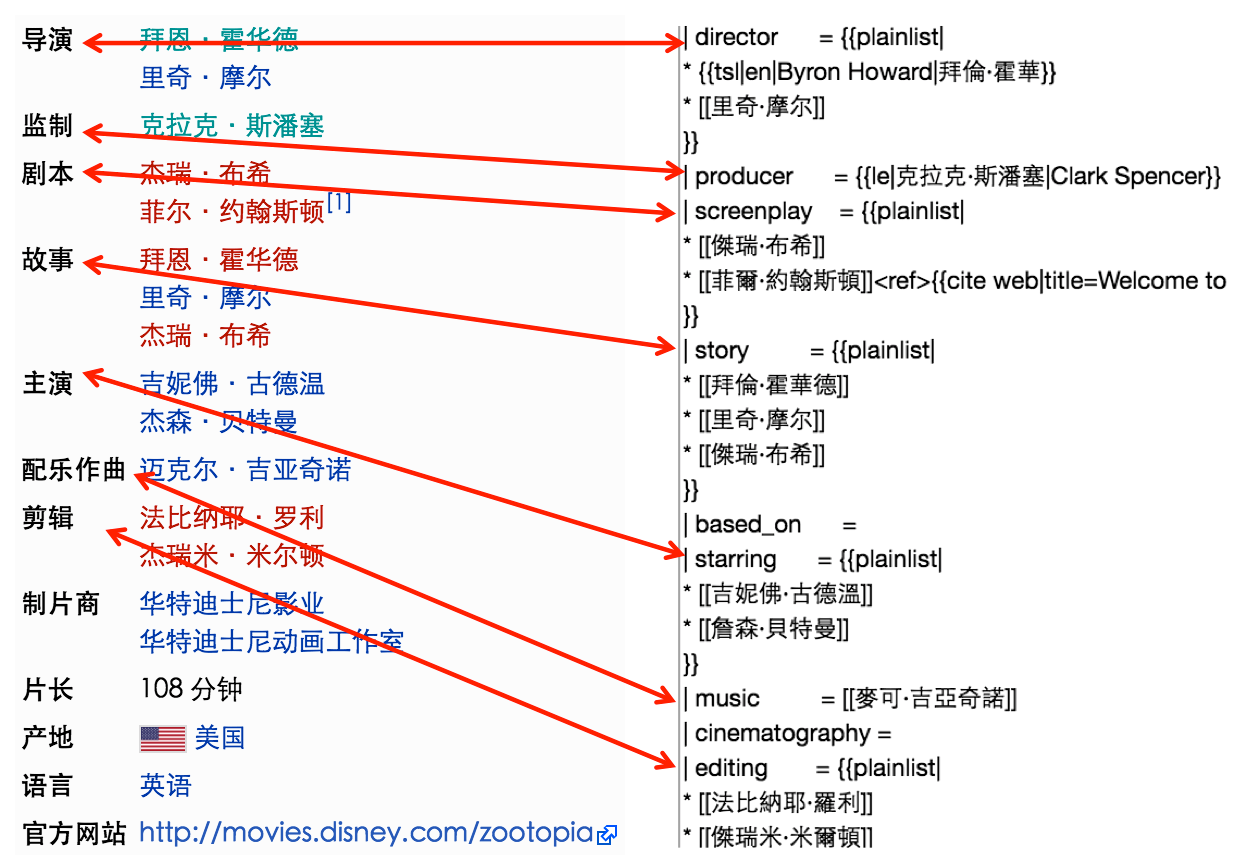
\includegraphics[width=0.8\columnwidth]{film-tl-rl}
  \caption{电影《疯狂动物城》模板标签与显示标签对比}
  \label{fig:film-tl-rl}
\end{figure}

而真实的模板是怎么定义的呢?模板在维基百科中也设计成一个词条,在维基article数据文件中,含有对模板词条的具体定义。模板词条标签以\textit{Template:}开头,大部分的信息框模板标签则以\textit{Template:Infobox}开头,但也有例外,在中文维基中,类似\textit{Template:电影信息框}等具有语言本地化特色的标签有很多。在之后的工作中,我们统计出以\textit{Template:Infobox}标识的模板占所有英文信息框模板的91\%,中文的63.5\%。由此可见,单纯通过词条标签来筛选出信息框模板并不是一个良策。

通过对模板内容进行总结,我们发现信息框模板的源代码中都含有\textit{infobox}字样,该infobox所涵盖的区域中,包含模板属性定义,可以认为带有infobox信息的Template为信息框模板。

尽管区分出信息框模板,模板中内容格式却不尽相同。根据版式特点,我们将信息框模板归为三类,分别为键值对模板、表格模板与继承模板,图\ref{fig:template-examples}给出三种模板示例,我们将在\ref{sec:property-extraction}中给出详细介绍。

\begin{figure}[ht]
\centering
    \begin{subfigure}{7.2cm}
        \centering
        \fbox{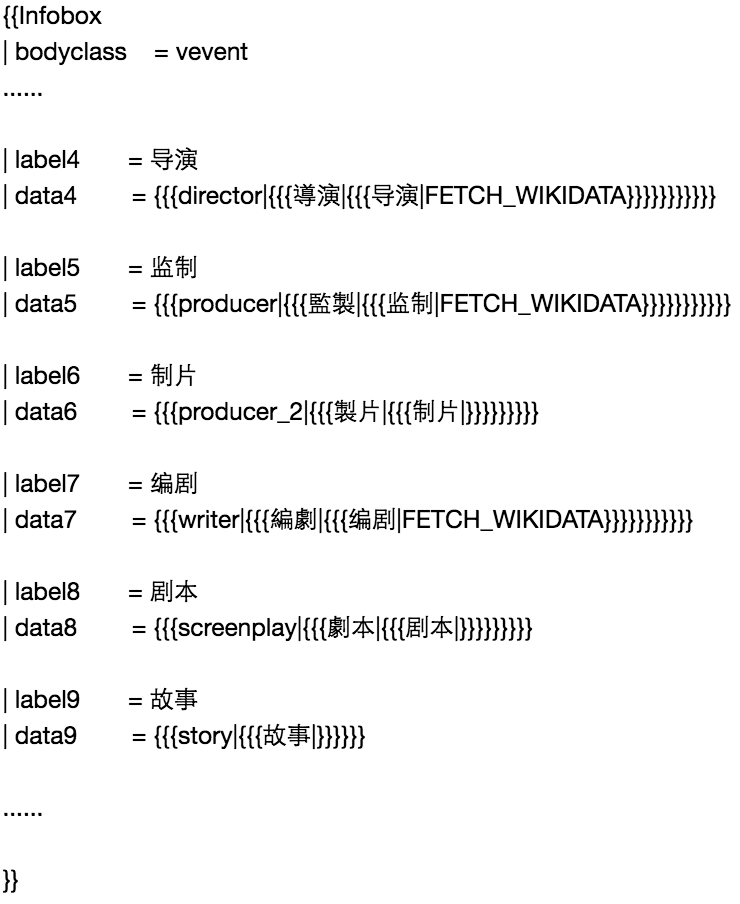
\includegraphics[width=0.8\textwidth,height=5.6cm]{template-keyvalue}}
        \caption{键值对模板示例}
        \label{fig:template-keyvalue}
    \end{subfigure}
    \hspace{0.01cm}
    \begin{subfigure}{7.2cm}
        \centering
        \fbox{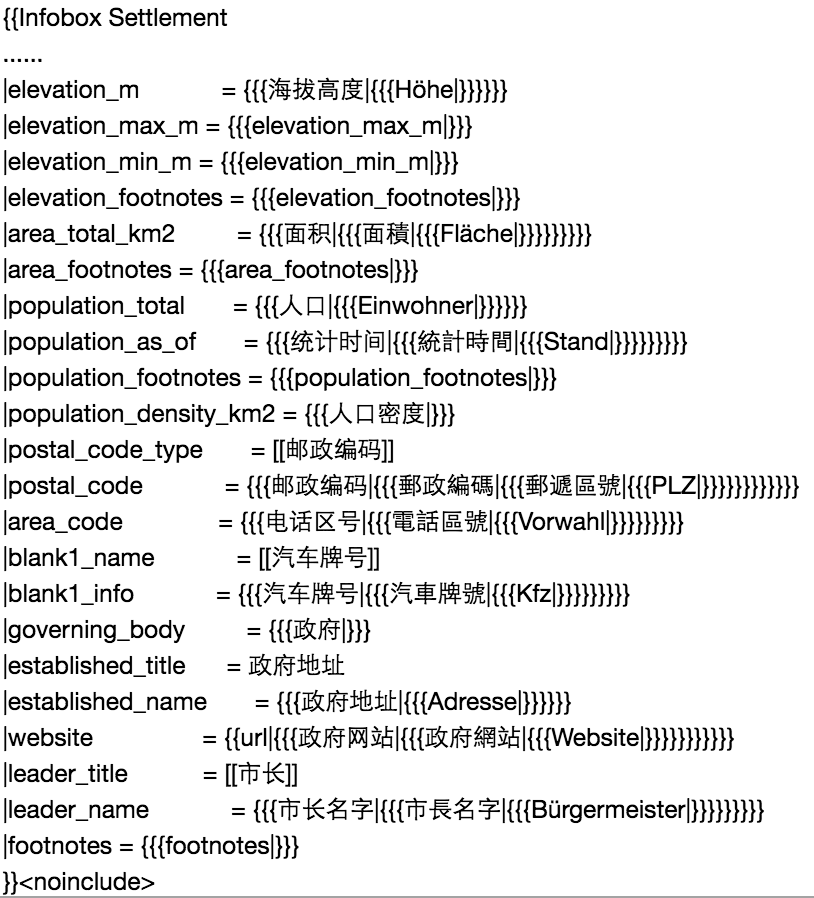
\includegraphics[width=0.8\textwidth,height=5.6cm]{template-inherit}}
        \caption{继承模板示例}
        \label{fig:template-inherit}
    \end{subfigure}
    \vspace{0.01cm}
    \begin{subfigure}{9.6cm}
        \centering
        \fbox{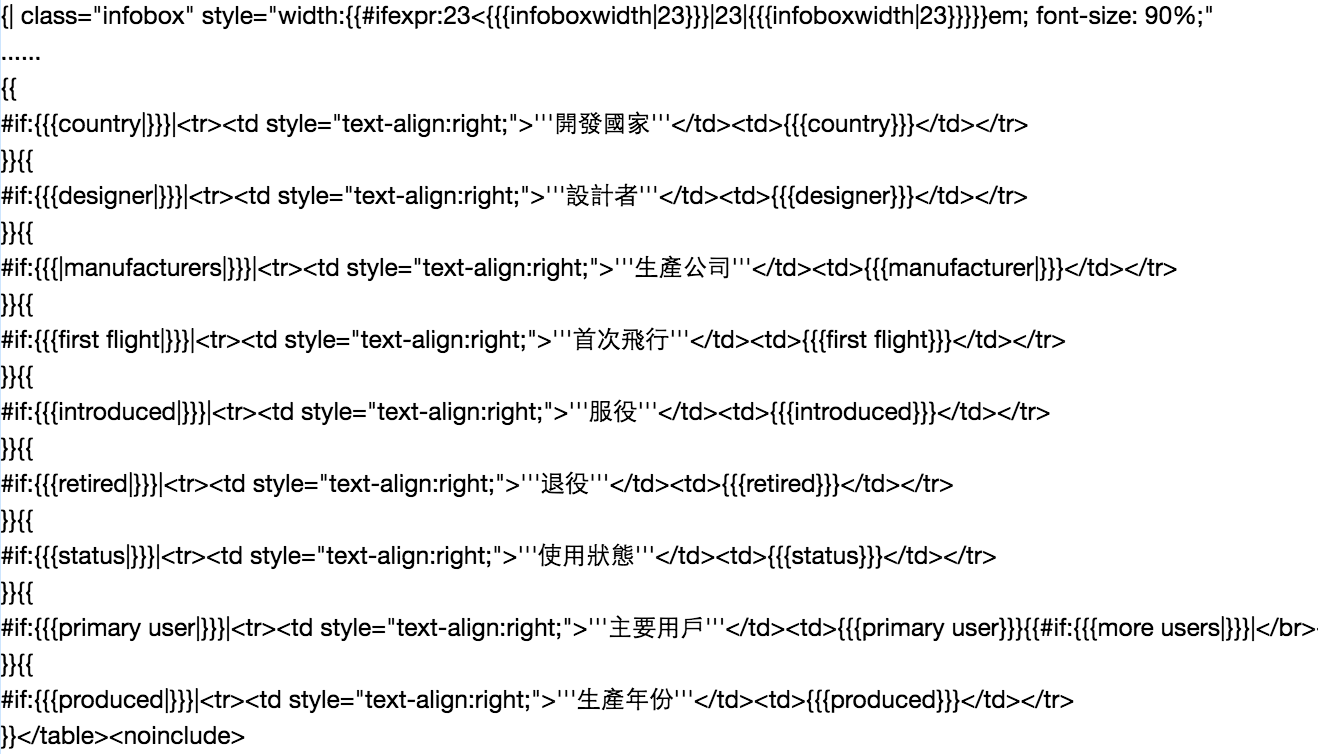
\includegraphics[width=0.8\textwidth]{template-table}}
        \caption{表格模板示例}
        \label{fig:template-table}
    \end{subfigure}
\caption{模板类型举例}
\label{fig:template-examples}
\end{figure}

除了以上三类,数据文件中还出现了{\heiti 重定向模板},内容如图\ref{fig:template-redirect}。该类模板的出现,是因为维基百科经过多次整理与更新,会将相似模板合并,或重新定义模板名称,被删除的模板会重定向到新模板上。2016年2月的中文维基上,\textit{Template:Infobox Film}与\textit{Template:Infobox film}都重定向到\textit{Template: 电影信息框}。

\begin{figure}[H]
  \centering
  \fbox{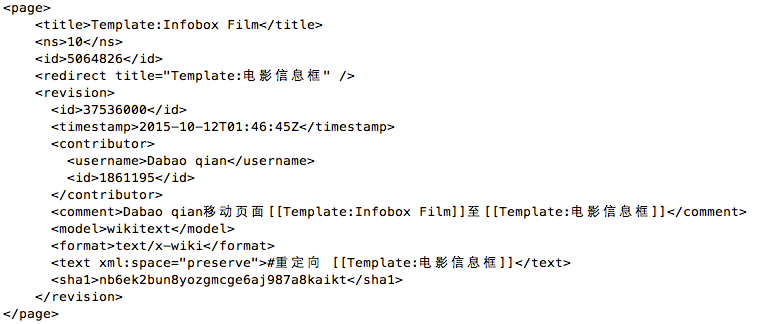
\includegraphics[width=0.75\columnwidth]{template-redirect}}
  \caption{重定向模板内容展示}
  \label{fig:template-redirect}
\end{figure}

\section{问题描述}

我们认为,一个指定的概念$c_i \in C$所代表的领域下,会有一个属性集合$P(c_i)=\{p_{i,j}|j=1,2,...,n\}$表征$c_i$中的所有实例$I(c_i)$的特性。我们定义概念属性$p_{c_i}= <c_i, label, I, V>$,表示其带有概念$c_i$的领域信息,只描述$i_{c_i} \in I(c_i)$。$label$表示属性标签,即使$p_{c_i}.label == p_{c_j}.label$,$p_{c_i} \neq p_{c_j}$。$I$代表$p_{c_i}$在$c_i$下描述的实例集合,$V$代表$p_{c_i}$的描述$I$的所有值集合。

本章的工作是从维基百科中生成概念属性。给定一个维基百科$W$,可以得到模板$T$,模板存储描述一类实例的属性集合,对于模板$t_i$,我们有$P(t_i)=\{p_{i,j}|j=1,2,...,n\}$。可以认为,模板代表着一类概念,则有$T \approx C$。

鉴于\ref{sec:template-analysis}中对模板与属性的分析,基于维基的概念属性,在定义上需要进行一些改动:
\begin{itemize}
\item 维基百科在数据文件中使用的属性标签,与现实在页面的不一致(图\ref{fig:film-tl-rl})。我们将数据文件中使用的标签定义为模板标签(template label),用$tl$表示,展示在页面上的称为显示标签(render label),用$rl$表示。则有$p_{c_i}.label = <tl, rl>$。
\item 维基百科的模板可能有相近或重复,此时所代表的概念是存在包含关系的。因此严格来说,有$c = \{t_i|i=1,2...n\}$。
\end{itemize}

具体到维基百科,本章工作抽象为:给定一个维基百科$W = <T>$,生成概念集合$C$,其中$c = \{t_i|i=1,2...n\}, c \in C, t_i \in T$,以及概念属性集合$\mathbb{P} = \{P(c_i)| i = 1,2,...,n\}$,其中对于$p_{c_i} \in P_{c_i}$,有$p_{c_i} = <c_i, tl, rl>$。

\section{概念属性生成}
\label{sec:property-extraction}

我们对三类信息框模板分别进行抽取,收集模板标签与显示标签的关系。我们发现,一个属性的显示标签,可能根据模板标签有所变化。抽取过程中,所有模板标签与显示标签的关系都会保留下来,我们以$<T, tl, rl>$的格式保留一组属性记录。

{\heiti 键值对模板($T_{kv}$)(图\ref{fig:template-examples}a):} 这种类型的模板,其显示标签与模板标签在infobox中以
%\begin{figure}[ht]
%\begin{center}
%\framebox[0.3\linewidth]{
%    \begin{minipage}[t]{0.25\linewidth}
%    label=显示标签\\
%    data=模板标签
%    \end{minipage}
%}
%\end{center}
%\end{figure}
\begin{center}
\verb"label=显示标签"

\verb"data=模板标签"
\end{center}
的格式存在。一个模板中,显示标签与模板标签的关系可能是一对一、一对多、多对多的,即一个属性根据不同的模板标签,可能会显示不同的标签在页面上。

{\heiti 表格模板($T_{table}$)(图\ref{fig:template-examples}b):}这种类型的模板以类似表格的形式对属性进行编排,抽取方法与键值对模板不同,根据表格行列思想,通过分析<td>等标签抽取。

{\heiti 继承模板($T_{inherit}$)(图\ref{fig:template-examples}c):}有半数左右的模板存在继承关系,即其模板标签的表示含义与父类模板相同,标签对应关系要结合父类模板来挖掘。继承模板可能继承自键值对模板、表格模板,甚至重定向模板。

{\heiti 重定向模板($T_{redirect}$)(图\ref{fig:template-redirect}):}对于分析实例对模板的应用情况至关重要,编辑者可能在编写信息框时用的旧版模板标签,或者不注意大小写。\ref{fig:template-redirect-examples}给出不同词条对同一模板的不同编辑方式。如果不考虑重定向模板标签,在前三类的基础上直接匹配,会大大影响已抽取模板对词条的覆盖率。因此重定向模板虽然没有实质内容,也不能弃之不理。

\begin{figure}[H]
  \centering
  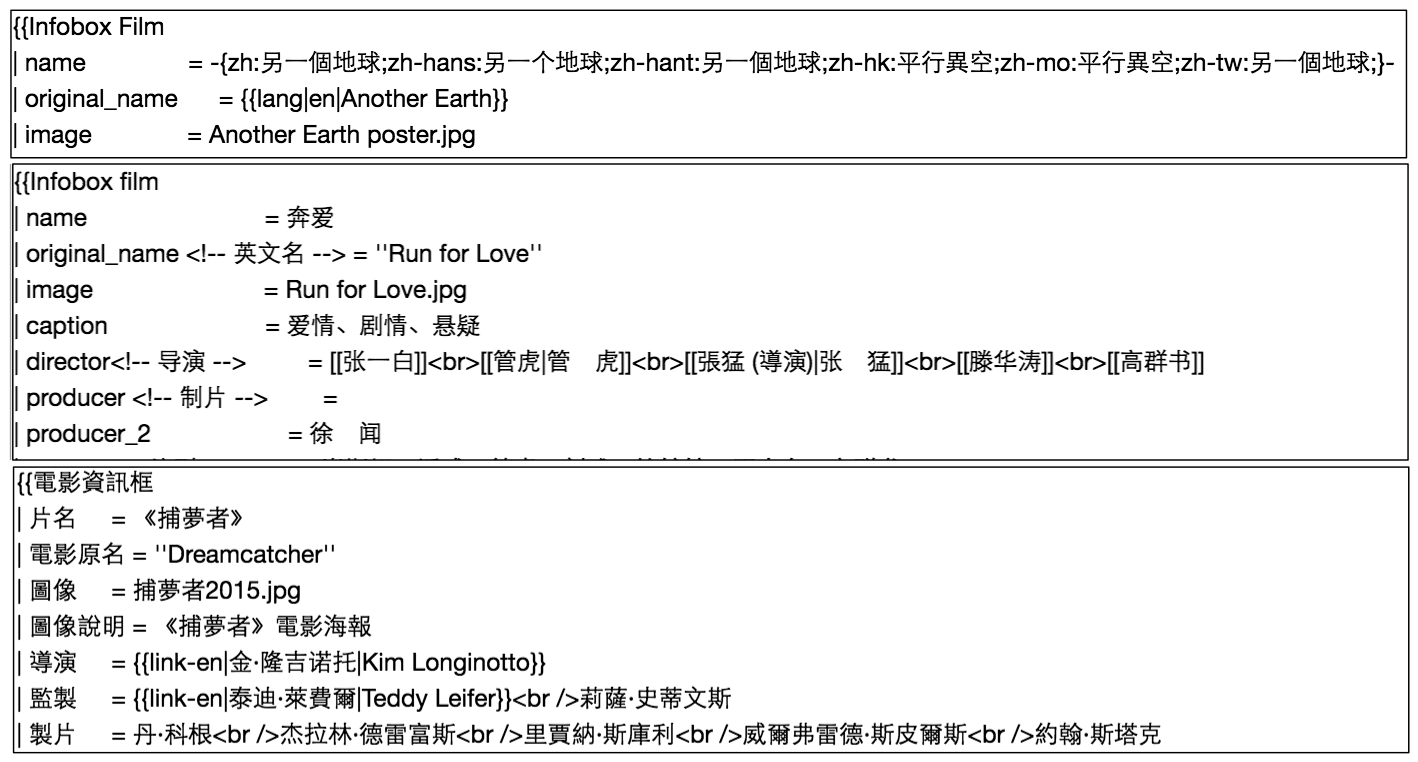
\includegraphics[width=0.8\columnwidth]{template-redirect-examples}
  \caption{重定向模板使用情况举例}
  \label{fig:template-redirect-examples}
\end{figure}

\subsection{结果统计}

基于以上四类信息框模板,我们对2016.03版本的英文维基与2016.02版本的中文维基分别抽取,表\ref{tab:wiki-infobox-statistic}是对当前维基现状的统计分析。

\begin{table}[htb]
    \centering
    \caption{中英文维基百科词条信息统计}
    \label{tab:wiki-infobox-statistic}
    \begin{tabular}{cccc}
    \toprule[1.5pt]
    {\heiti 维基百科} & {\heiti 词条数} &  {\heiti 含有信息框的词条数及比例} & {\heiti 使用模板数} \\\midrule[1pt]
    英文维基 & 5,138,426 & 2,344,305(45.6\%) & 4491 \\
    中文维基 & 863,918   & 261,045(30.2\%)   & 2317  \\
    \bottomrule[1.5pt]
    \end{tabular}
\end{table}

得到各类型信息框模板数量如表\ref{tab:infobox-template}所示

\begin{table}[htb]
  \centering
  \caption{各类型信息框模板数量}
  \label{tab:infobox-template}
  \begin{tabular}{cccccc}
  \toprule[1.5pt]
      {\heiti 维基百科} & {\heiti 键值对} &  {\heiti 表格类} & {\heiti 集成类} & {\heiti 重定向} & {\heiti 总数}\\\midrule[1pt]
      英文维基 & 1910 & 1901 & 1897 & 4076 & 9784\\
      中文维基 & 840  & 878  & 968  & 956  & 3642\\
  \bottomrule[1.5pt]
  \end{tabular}
\end{table}

我们对各模板进行了分析,因为数据杂乱等原因,我们无法成果获取所有模板中的信息,而是以常用模板为优先,并以词条覆盖率90\%以上为目标结束属性生成任务。成功解析的属性信息如表\ref{tab:render-label}所示,其中不包括对重定向模板的解析。

\begin{table}[htb]
  \centering
  \caption{概念属性信息生成结果}
  \label{tab:render-label}
    \begin{tabular}{ccccc}
    \toprule[1.5pt]
      {\heiti 维基百科} & {\heiti 模版数} & {\heiti 模板中属性数} & {\heiti 属性/模板}  &{\heiti 模板标签/属性} \\\midrule[1pt]
      英文维基 & 3819 & 104741 & 27.45 & 1.27  \\
      中文维基 & 1895 & 44797  & 23.64 & 1.34  \\
    \bottomrule[1.5pt]
    \end{tabular}
\end{table}

我们在\ref{tab:coverage}中给出当前生成的概念属性对维基百科的覆盖程度。实际使用的模板名称与模板正式名称的匹配率较低,需要经过一系列转化,包括:大小写转换、去除多余空格、重定向模板转换等。
模板覆盖率为抽取出的模板数量与所有词条使用的全部模板数量的占比,模板属性覆盖率为所有抽取出的模板属性对所有词条的所有属性数量的占比,词条覆盖率为能用抽取模板分析的词条的百分比,我们获取的概念属性可以处理90\%以上的维基词条的信息框。

\begin{table}[htb]
  \centering
  \caption{结果覆盖率统计}
  \label{tab:coverage}
    \begin{tabular}{cccc}
      \toprule[1.5pt]
      {\heiti 维基百科} & {\heiti 模板覆盖率} & {\heiti 模板属性覆盖率}  & {\heiti 词条覆盖率} \\\midrule[1pt]
      英文维基 & 87.6\% & 27\% & 96.7\%  \\
      中文维基 & 77.8\% & 33\% & 90.3\%  \\
      \bottomrule[1.5pt]
    \end{tabular}
\end{table}

\ref{tab:template-examples}给出了常用模板举例,\ref{tab:template-property-examples}给出了三个常用中文模板的部分属性举例。

\begin{table}[htb]%建议把模版名中的infobox删掉
  \centering
  \caption{常用模板统计}
  \label{tab:template-examples}
    \begin{tabular}{llll}
    \toprule[1.5pt]
    \multicolumn{2}{c}{\heiti 英文维基}   & \multicolumn{2}{c}{\heiti 中文维基} \\
       模版名称&使用频次&模版名称&使用频次 \\\midrule[1pt]
       Infobox settlement   & 253276 & Infobox Settlement & 34717 \\
       Infobox person       & 158481 & 艺人 & 14047 \\
       Infobox football biography & 127402 & Infobox Planet& 12163 \\
       Infobox film         & 102863 & 文物保护单位& 10362 \\
       Infobox officeholder & 86698 & Infobox officeholder& 7501\\
       Infobox album        & 77436 & Infobox French commune& 7297\\
       Infobox musical artist & 74469 & 电影信息框& 6787 \\
       Infobox company      & 46646 & Infobox person& 6414 \\
       Infobox NRHP         & 42385 & 电视节目信息框& 5958\\
       Infobox single       & 40578 & Infobox Company& 5138 \\
    \bottomrule[1.5pt]
    \end{tabular}
\end{table}

\begin{table}[htb]%显示里的[[]]有必要保留吗?
  \centering
  \caption{常用模板属性举例}
  \label{tab:template-property-examples}
  \begin{tabular}{llllll}
      \toprule[1.5pt]
        \multicolumn{2}{c}{\heiti 艺人}  & \multicolumn{2}{c}{\heiti Planet} & \multicolumn{2}{c}{\heiti 电影}\\
        模板标签& 显示标签 & 模板标签& 显示标签& 模板标签& 显示标签\\ \midrule[1pt]
        Alias & 昵称      & discovered & 发现日期      & budget & 预算 \\
        hometown& 籍贯    & discoverer & 发现者        & director & 导演\\
        URL& 网站         & density & 平均[[密度]]     & producer& 监制 \\
        child& 儿女       & mass & [[质量]]            & writer & 编剧\\
        children& 儿女    & inclination & [[轨道倾角]] & starring & 主演\\
        country & 国籍    & named\_after& 命名依据     & music &  配乐作曲\\
      \bottomrule[1.5pt]
  \end{tabular}
\end{table}

%\section{概念合并}
%
%最后我们有xx个概念,共xx个属性
%
\section{本章小结}

本章主要从维基百科中生成概念属性。我们将维基模板相关的领域视为概念,其中的属性视为该概念下的属性,并用\textit{属性@模板}的方式定义一个属性,这种方法同时可以解决属性多义问题,即认为同一领域下的属性没有歧义性。

为了获得尽可能多的概念属性,我们对维基百科模板和属性进行了细致的分析,将模板分为键值对模板、表格模板、继承模板与重定向模板,分别进行处理,将属性赋予模板标签与显示标签两种信息,这些工作,有助于他人对于属性和模板有更深入的理解。


\chapter{基于异构百科的跨语言属性对齐}
\label{cha:property-matching}

\section{本章引论}
维基百科是全球最大的百科数据库,目前支持228个语言。因语言差异、地域区别等多种原因,英文维基词条与信息框数量远超其他语言,信息量很不对称。仅以中英文维基为例,如图\ref{fig:en-zh-article-infobox-compare}所示,截止到2016年2月,英文维基词条约是中文维基的6倍,包含信息框的词条数更是高达9倍。中英文维基数据,尤其在信息框数据,的严重不平衡性,使得基于维基百科构建的中英文知识库缺少足够的属性链接。

\begin{figure}[h]
  \centering
  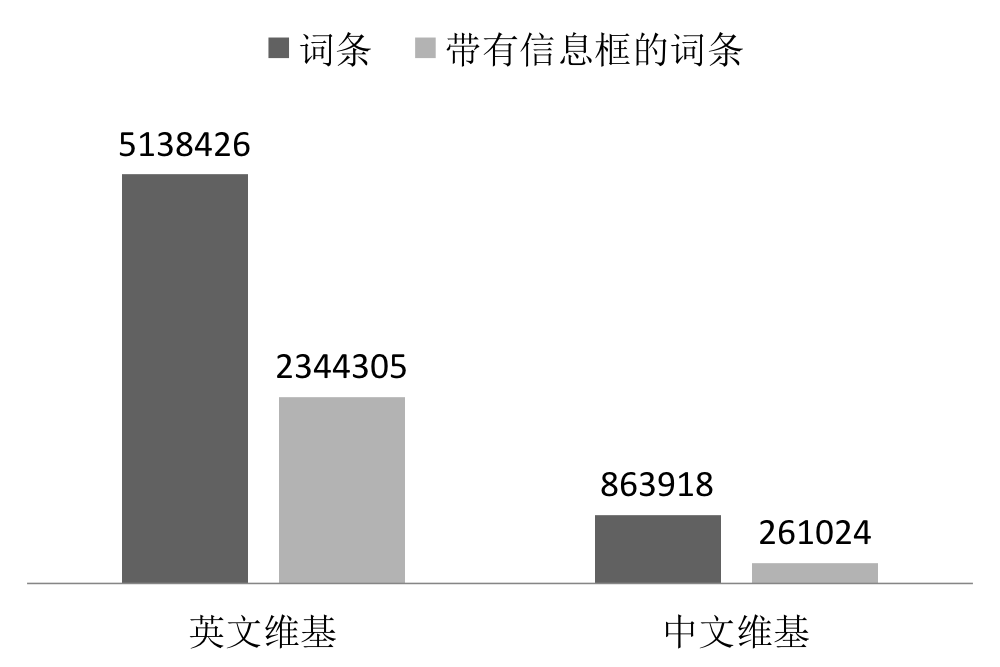
\includegraphics[width=0.6\columnwidth]{en-zh-article-infobox-compare}
  \caption{中英文百科词条数量对比}
  \label{fig:en-zh-article-infobox-compare}
\end{figure}

%维基百科中中英文数据的不平衡,尤其在信息框上差距更加显著,使得基于维基百科构建的中英文知识库缺少足够的属性链接。

而百度百科作为中国活跃的开放式网络百科之一,参与人数众多,信息较为全面。截止到2014年12月含有信息框的词条数量达到xxx。图\ref{fig:frozen-infobox}对比了中英文维基和百度百科中电影《冰雪奇缘》的信息框内容,可以发现三个百科信息各有异同,能够互相补充。如果能充分利用它们之间的关系,比如通过百度百科的信息框补全中文维基信息框、利用中文维基与英文维基的对齐关系找到英文维基与百度百科的对齐关系等,就可以进一步促进知识补全,实现中英文知识融合。

本章从抽取更多跨语言知识,融合异构百科的角度出发,引入具有丰富中文信息的在线百科,发现百度百科与英文维基百科的中英文属性对齐关系。这是一个跨语言、跨异构百科的任务,就我们所知,当前还没有自动抽取百度百科属性信息,并与维基百科知识对齐的工作。

我们的工作面临跨语言与跨异构百科两项挑战,对于前者,因为维基百科与百度百科相互独立,在词条、分类乃至信息框属性方面,并没有直接的跨语言链接,如果能增加两者的关联信息,跨语言对齐的研究将会更加得心应手。对于后者,编辑规则的迥异,给同语言的对齐工作也带来障碍。本章根据维基百科与百度百科的异同,提出跨语言属性对齐框架,力图获得中文同语言的同义关系与跨语言的对齐关系。


\section{问题描述}
本章的工作致力于解决中英文异构百科的跨语言信息框属性对齐问题。图\ref{fig:frozen-infobox}为电影《冰雪奇缘》在维基百科与百度百科中的信息框对比图,从左到右别为中文维基、英文维基、百度百科中的信息框。本章任务则是将指代同一个实体的中英文词条$a_e,a_z$中两个信息框中描述相同特性的属性匹配,比如\textit{Starring}对\textit{主演},\textit{Directed by}对\textit{导演}。

\begin{figure}[H]
  \centering
  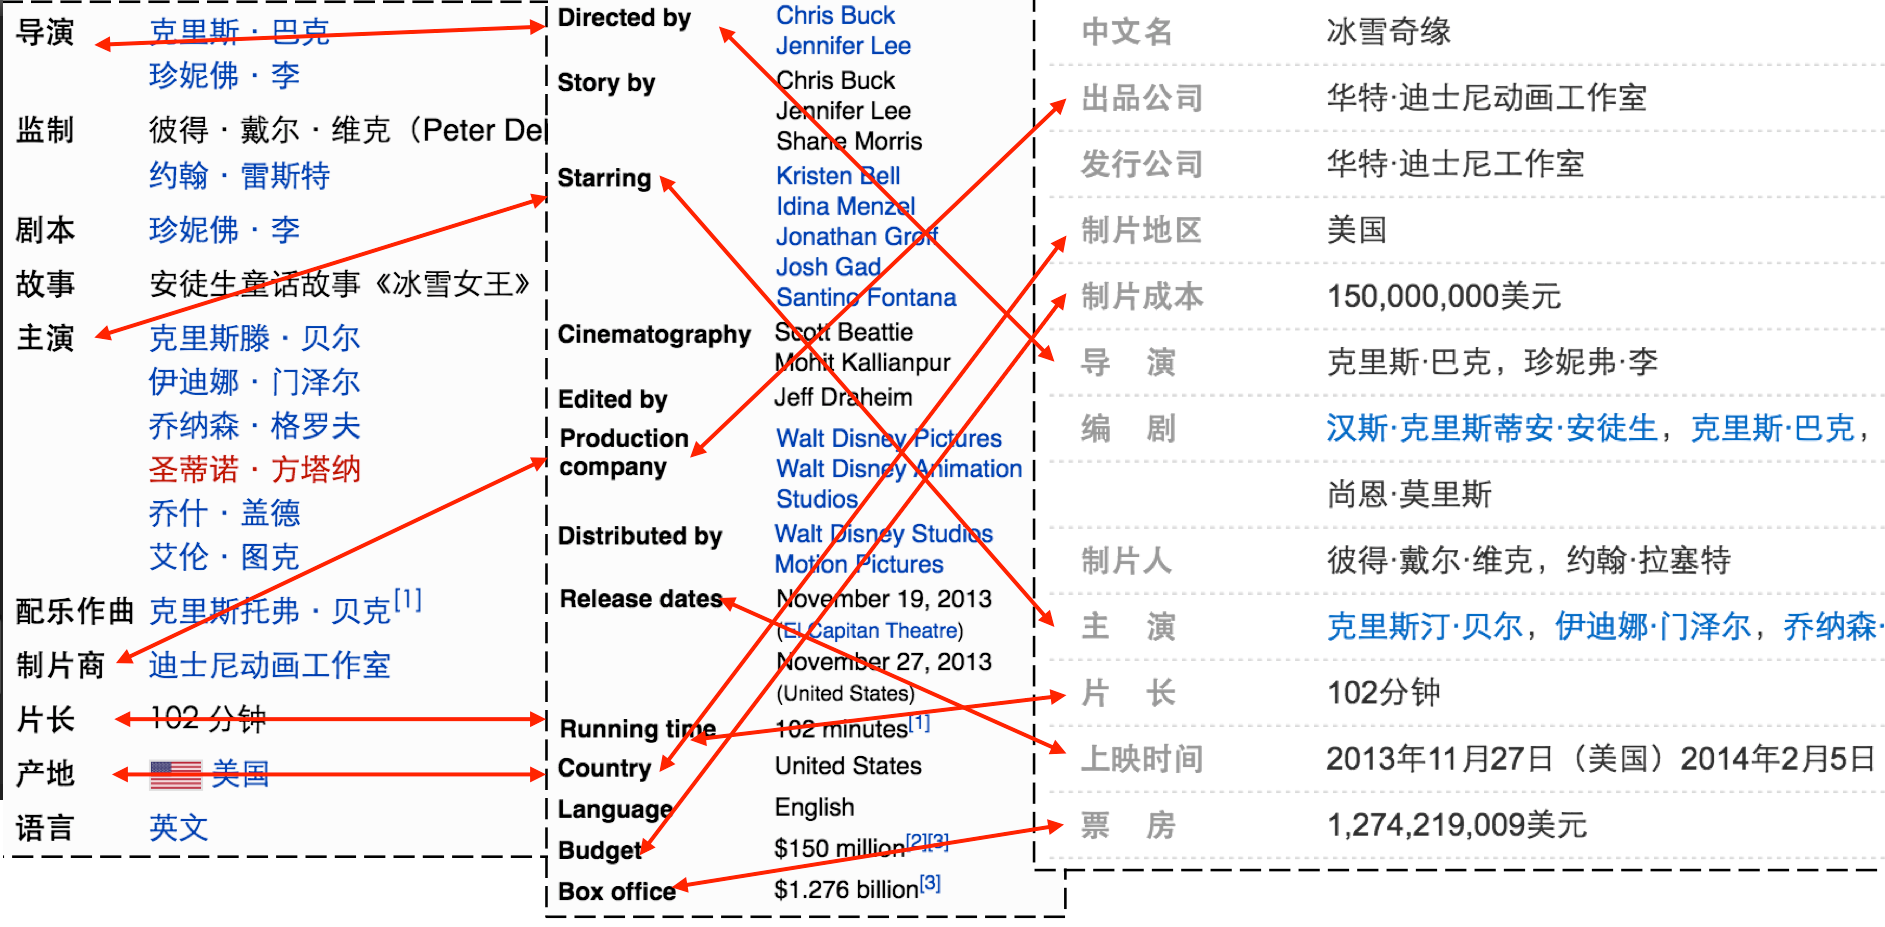
\includegraphics[width=0.9\columnwidth]{frozen-infobox}
  \caption{中英文信息框属性对齐示例}
  \label{fig:frozen-infobox}
\end{figure}

我们引入第\ref{cha:concept-property}章中的{\heiti 概念模板},认为属性在特定概念下的含义是唯一的,同时将对属性的分析限制在概念领域范围内,属性的同义词查找、跨语言链接等,都在同一领域里进行。为此,首先需要确定一个概念$c \in C$,并生成该概念下的属性集合(模板)$P(c)=\{p_1,...p_n\}$。
其中每个概念$c$下都包含一组词条$A(c)$,$p_c$只能描述$c$的词条,对一个指定的属性$p_c$,其所描述的词条集合为$A(p_c)$,$A(p_c) \subseteq A(c)$。此外,对于每个带有属性$p_c$的词条$a(p_c) \in A(p_c)$,都有一个对应属性值$a(p_c).v$。

基于上述概念,跨语言信息框属性对齐问题可定义为:
\begin{definition}
给定对应的中英文领域$c_e \in C_E \leftrightarrow c_z \in C_Z$,找到其中的跨语言对齐属性对$p_{c_e} \leftrightarrow p_{c_z}$。
\end{definition}

\section{异构百科的模板与属性分析}
\label{sec:template-property-analysis}

基于异构百科的跨语言属性对齐工作,除了语言差异的挑战,另一个挑战则是来自于维基百科与百度百科的异构性。

各个百科鼓励编辑者使用模板对词条进行组织与编辑。信息框的编辑也由模板来规范,比如百度百科中,描述人物使用\textit{人物通用模板};维基百科中,电影使用\textit{Template:电影信息框}。与此同时,用户在模板信息项之外,可自行添加自定义属性,丰富信息框内容,使其个性化。

利用模板信息,我们可以获得大量的属性集合以及属性与概念领域的对照关系。理想情况下,只要能找到跨语言下的异构百科中模板的对应关系,就能获得相关的属性的对齐关系,达到跨语言、跨百科属性对齐的目标。但是实际上,这个过程存在诸多阻碍:
\begin{itemize}
\item {\heiti 百度百科模板无法获取。} 百度百科数据用于商业用途,没有像维基百科一样公开数据,因此其数据的获取多来源于网络爬虫。虽然网页涵盖了词条的几乎所有内容,但并不包含编辑信息,比如模板的使用。因此我们只能获得百度百科的属性集合,并依赖进一步的研究分析,猜测模板内容。
\item {\heiti 异构百科定义的模式不同。} 姑且不说中英文差异,单是中文维基与百度百科,在对同一概念下词条的描述,命名规范与侧重点都不尽相同。以电影领域模板为例,图\ref{fig:frozen-infobox}中可以看到,中文维基使用\textit{制片商},百度百科使用\textit{出品公司}作为电影制作公司属性的标签,可见{\heiti 属性多义性}。另一方面中文维基包含\textit{旁白}、\textit{配乐作品}等百度百科不使用的属性,百度百科包含\textit{imdb编码}等维基模板中没有的属性,可见{\heiti 模板缺失性}。若想尽可能保留属性集合的完整度,保证准确度,我们需要处理属性多义与模板缺失问题。
\end{itemize}

模板的差异,为属性对齐工作带来了更多的困难,但这也表明异构百科下属性的使用,确实有值得探究之处。我们可以通过寻找同一种属性在异构百科下的不同表达方式,寻找相似属性名称;融合多个百科的属性集合,获得概念下更全面的属性集合,生成通用模板。

\section{基于异构百科的跨语言属性对齐}
\label{sec:property-matching}

本章致力于解决跨语言概念属性的对齐,由于数据的不规范,我们需要解决百度百科概念属性生成、同义属性合并等诸多问题。

%本任务获得的领域下的属性模板,可以避免人工构建模板,有助于增加信息框的有意信息,查漏补缺,另一方面,获得属性同义表达方式,可以为融合其他百科信息做铺垫。属性模板的构成、属性的分布、属性的命名,在一定程度上都可以对用户行为分析、文本分析做贡献。比如一个实体的关键信息都有什么、用户一般关注什么重点信息、人们多属性的常用称呼都有什么等等。一旦拥有属性模板,我们可以用自动化的方法,从文本中抽取相应的信息,自动构建词条信息框。[引用][][]中都在已知属性集合的基础上,对缺失属性进行填充。

图\ref{fig:property-matching}为整个跨语言属性对齐的框架图,根据前文所提出的问题,主要分为概念属性生成、同语言属性对齐与相似属性合并、跨语言种子集合生成、跨语言属性对齐四大模块。

\begin{figure}[h]
  \centering
  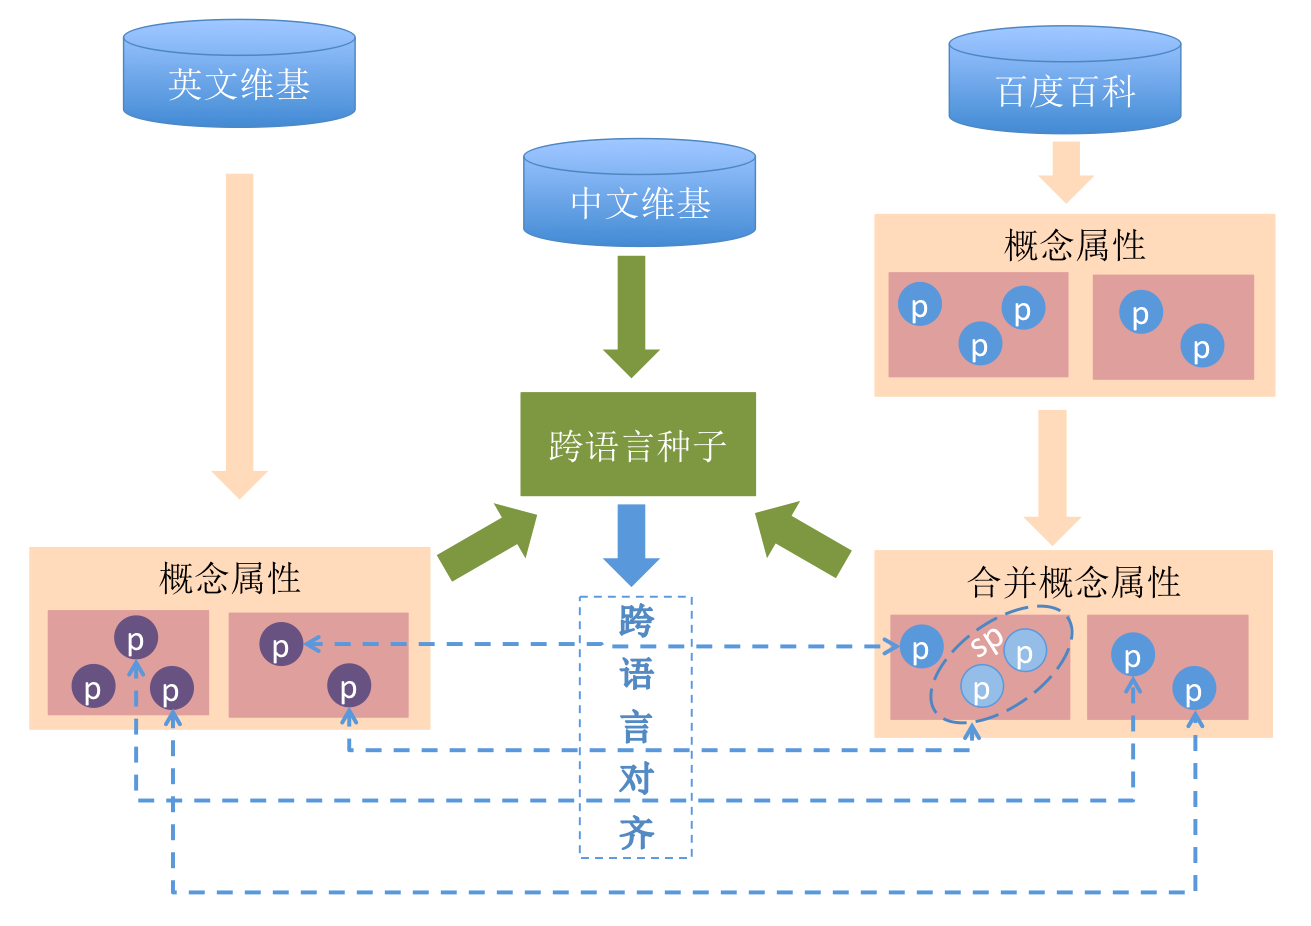
\includegraphics[width=0.78\columnwidth]{property-matching}
  \caption{跨语言属性对齐框架图}
  \label{fig:property-matching}
\end{figure}

本章数据基于第\ref{cha:concept-property}章中的结果数据,以及从2014年12月版本的百度百科网页上获取的信息。不同于维基百科复杂的概念属性抽取,百度百科页面不含模板信息,属性信息只能通过网页解析获得,具体过程不再赘述。

{\heiti 百度百科概念模板生成:}针对百度百科没有信息框模板的问题,我们根据属性词频与共现率,提出概念属性生成模型,旨在对给出的维基概念,在百度百科中模拟出对应的概念与概念属性集合,进而形成模板。概念属性集合,可作为今后编写信息框的参照,同时可看作属性对齐的候选集,大大减小了计算空间。

{\heiti 同语言属性对齐与相似属性合并:}针对属性的一义多词问题,即描述相同意义的属性,有不同的显示标签。
%我们从文本相似度、语义形似度等角度出发,计算获得特定属性的同义属性。
我们通过对齐中文维基与百度百科属性,找出高质量的属性同义词,有助于提高跨语言对齐的召回率。

{\heiti 跨语言种子集合:}维基百科与百度百科这两个异构百科没有直接的关联关系,但以中文维基为桥梁,并利用维基的跨语言特性,我们找到百度百科与中英文维基百科的联系,抽取出一部分高准确度的属性对齐关系。
%信息框属性在维基百科中,不像分类与词条一样含有显性的语言链接,不能直接获取,但我们依然可以通过信息框模板与词条链接等现有关系,抽取出正确的属性跨语言对齐关系。
%另一方面,通过分析同语言百科,获得对齐的中文属性集合。两两融合后,获得英文维基-中文维基-百度百科的属性对齐关系,形成跨语言种子集合。

{\heiti 跨语言属性对齐:}种子集合只包含小部分常用且识别度高的属性对齐关系,对于剩下的长尾问题,我们训练一个二元分类器,判断给定的中英文属性对是否为对齐关系。其中特征主要从文本、结构中抽取。

\subsection{百度百科概念模板生成}
\label{sec:domain-template}
根据模板的定义,我们假设一个概念领域中使用频率高且在其他领域极少出现的属性为该领域的代表属性。该思想与TF-IDF(Term Frequency–Inverse Document Frequency)相近,属性的TF-IDF表征其对于某一概念的重要程度。

如何界定一个概念及其相关信息?在第\ref{cha:concept-property}章中,我们认为模板规范着一类词条的编辑,关联着一个概念领域,即$T \approx C$。第\ref{cha:concept-property} 章中抽取的信息框模板覆盖了90\%的维基文档,可以认为涵盖了百科中的大部分领域。由于英文维基的模板已知,当前的任务可以定义为:给定来自英文维基的概念$C_E$,在百度百科$W_b$中抽象出与其对应的中文概念$C_Z$,及其属性集合$P(C_Z)={p_1^z,...,p_n^z}$。其中,不同于$C_E$由明确的模板组成,$W_b$中的$C_Z$是一个抽象存在,可以认为$P(C_Z)$就代表着$C_Z$中实例的特性,组成概念领域$C_Z$的模板。

哪些属性可以涵盖在$C_Z$内?我们首先获取$P(C_Z)$的候选集。根据百科的结构,可以通过直接关联找到关系密切的属性,并利用间接关系扩展属性候选:

{\heiti 直接关联:} $C_E$中的词条$A(C_E)$对应的跨语言词条集合$A_Z$使用的属性,认为是与$C_E$直接关联的属性,定义为$p_{direct}$;

{\heiti 间接关联:} $C_E$中的词条$A(C_E)$涉及的分类$Ca(C_E)$对应的跨语言分类集合$Ca_Z$下,对应词条$A_Z'$使用的属性,认为是与$C_E$间接关联的属性,定义为$p_{indirect}$。考虑到维基分类体系的不完善,可能引入不相关的分类导致其他领域的词条混入,我们对$Ca$进行了筛选,具体来说:

\begin{equation}
Ca(C_E) = Top_k\{ ca_i\mid |A(ca_i)| > 2 \}
\end{equation}
即$Ca$必须含有2个以上的词条,且只取包含词条数量最多的前$k(k=10)$个分类。

接下来,我们通过计算属性的TF-IDF来度量其对给定概念的标识度,即:
\begin{align}
\label{equ:tf}
tf_{i,j}=\frac{n_{i,j}}{\sum_{k}{n_{k,j}}}
\end{align}
\begin{align}
\label{equ:idf}
idf_{i}=1+log\frac{\left | D \right |}{\left | j:t_i  \epsilon d_j \right |}
\end{align}
\begin{align}
\label{equ:tfidf}
tfidf_{i,j}=tf_{i,j}\times idf_{i}
\end{align}

\ref{equ:tf}中$n_{i,j}$是属性在领域$d_{j}$中的使用频次,分母则是在领域$d_{j}$中全部属性的使用次数之和。对属性频次的计算,因为直接关联属性比间接关联属性更重要,权值应更高,因此

\begin{align}
n_{i,j} = {\sum_{k}{x_{k,j}}}
\end{align}

\begin{align}
x_{k,j} =
\left\{\begin{matrix}
2 & p_i = p_{direct} \ in \ d_j\\
1 & p_i = p_{indirect} \ in \ d_j\\
0 & p_i \ not \ in \ d_j
\end{matrix}\right.
\end{align}

%\subsubsection{结果}
表\ref{tab:baidu-template-examples}给出两个典型概念下属性集合。

\begin{table}[htb]
  \centering
  \caption{百度百科概念模板生成结果举例(前20)}
  \label{tab:baidu-template-examples}
    \begin{tabular}{cccc}
      \toprule[1.5pt]
         \multicolumn{2}{c}{Planet} & \multicolumn{2}{c}{电影信息框}\\ \midrule[1pt]
         发现者   &  自转周期  & 导演     & 其他译名 \\
         发现时间 &  离心率    & 制片地区 & 外文名   \\
         中文名   &  绝对星等  & 片长     & 出品时间 \\
         质量     &  反照率    & 主演     & 出品公司 \\
         公转周期 &  平近点角  & 上映时间 & imdb编码 \\
         分类     &  别称      & 对白语言 & 制片人   \\
         直径     &  半长轴    & 类型     & 分级     \\
         外文名   &  平均密度  & 编剧     & 发行公司 \\
         发现日期 &  表面温度  & 色彩     & 拍摄日期 \\
         倾倒斜角 &  天体名称  & 中文名   & 拍摄地点 \\
      \bottomrule[1.5pt]
    \end{tabular}
\end{table}


\subsection{同语言对齐与相似属性合并}
\label{sec:similar-property}

以中文维基为桥梁实现英文维基与异构百科的关联的首要任务是尽可能找出同语言下的属性关系。本小节通过对中文维基与百度百科的信息框属性分析,解决1)同语言属性对齐和2)相似属性查找两个问题。

同语言属性对齐基于多策略提取,具体来说:
\begin{enumerate}%[策略1]
\item {\heiti 基于属性名称:}   描述同一实体的两个百科词条中,如果信息框属性名称一致,认为是同一属性;
\item {\heiti 基于相同属性值:} 描述同一实体的两个百科词条中,如果信息框属性名称有相同字符,且属性值相同,则认为是同一属性;
\item {\heiti 基于相似属性值:} 描述同一实体的两个百科词条中,如果信息框属性属性值相似,则认为是同一属性。为保证准确性,我们添加置信度衡量标准,即相似出现频率超过$N$次($N=5$)。
\end{enumerate}
表\ref{tab:zhwiki-baidu-cross-lingual}给出了不同策略的对齐数量和对齐属性举例。

\begin{table}[htb]
  \centering
  \caption{中文维基与百度百科属性对齐结果}
  \label{tab:zhwiki-baidu-cross-lingual}
    \begin{tabular}{ccc}\toprule[1.5pt]
      {\heiti 对齐方法} & {\heiti 数量} &  {\heiti 举例} \\\midrule[1pt]
      基于属性名称   & 2324 & Template:Infobox Game   [[游戏发行商|发行商]]   发行商  \\
      基于相同属性值 & 2365 & Template:Infobox Game   适用年龄    年龄 \\
      基于相似属性值 & 3781 & Template:Infobox scientist  获奖    主要成就  \\
      总数           & 8470 & -  \\
      \bottomrule[1.5pt]
    \end{tabular}
\end{table}

因为个人编写习惯,百科监管不严格等问题,属性可能有多种表达方式。我们在对齐结果中,发现中文维基一个属性可能对应多个百度属性标签,比如电影概念下,\textit{剪辑}有\textit{剪辑},\textit{剪辑导演},\textit{剪接}等不同表示方法。

如果一个属性有多个表示方法,应该将其视为一个属性。我们将代表相同含义但不同标签的属性合并成一个超属性$sp=\{p_1,...,p_n\}$。百度百科的每个属性都由$sp$来表示,如果某属性没有多形式表达,则$sp={p}, \left|sp \right|=1$。

本节中的同语言对齐方法较为严格,准确率较高,一对多情况下抽象出的$sp$可以直接利用。因为对齐结果较少,我们对其进行了人工验证,准确率在xxxxxx。

为寻找更多的相似属性,还可以进一步通过文本、值域、结构等特征对属性聚类。在理想情况下,一个类簇可以表示一个超级属性。我们尝试从文本相似度、Word2Vec语义相似度、值相似度三个维度特征入手,对百度百科同一领域的属性进行聚类。以\textit{电影(film)},\textit{公司(company)}, \textit{歌曲(single)}三个领域的结果进行评价,并与对齐方法进行对比,表\ref{tab:similar-property-compare}给出了对比结果。

\begin{table}[htb]
  \centering
  \caption{方法对比结果}
  \label{tab:similar-property-compare}
    \begin{tabular}{ccccc}
    \toprule[1.5pt]
      {\heiti 方法} & {\heiti 准确率} & {\heiti 召回率} & {\heiti 相似属性数量} & {\heiti 超属性数量($|sp|>1$)} \\\midrule[1pt]
      基于同语言对齐 & 1 & 1 & 1 & 1 \\
      聚类方法       & 1 & 1 & 1 & 1 \\
      \bottomrule[1.5pt]
    \end{tabular}
\end{table}

通过对比我们发现,基于聚类方法的同语言对齐,虽然在对齐数量上有明显增加,提高了召回率,但准确率却有所损失。超属性作为之后跨语言对齐的对象,其存在的瑕疵会造成错误累加,因此对其质量要求很高。基于此,我们使用同语言对齐时获得的相似属性结果,以保证之后工作的高质量。

\subsection{跨语言属性种子集合生成}
\label{sec:cross-lingual-seed}
我们采用间接对齐的方法寻找高质量跨语言属性对齐种子,即首先依赖维基百科跨语言特性,抽取中英文属性对齐关系,并以此为媒介寻找英文维基与百度百科的属性对齐关系。该过程可分为三个子步骤,即分别构建中英文维基百科、中文维基与百度百科、英文维基与百度百科的属性对齐关系。其中第二步在\ref{sec:similar-property}节中已有结果,在此不做赘述。

{\heiti 中英文维基百科跨语言属性对齐}在维基的语言链接,即现有跨语言模板与跨语言词条基础上实现。具体来说,分为三种情况,图\ref{fig:cross-lingual-seed}给出了较为直观的展示:

\begin{figure}[h]
%  \centering%
%  \begin{subfigure}{0.48\textwidth}
%    \centering
%    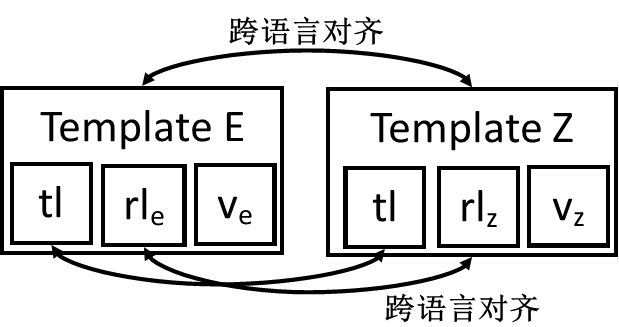
\includegraphics[width=0.8\textwidth]{enwiki-zhwiki-property-crosslinks-1}
%    \caption{基于跨语言模板对齐}
%  \end{subfigure}%
%  \hspace{0.01cm}%
%  \begin{subfigure}{0.48\textwidth}
%    \centering
%    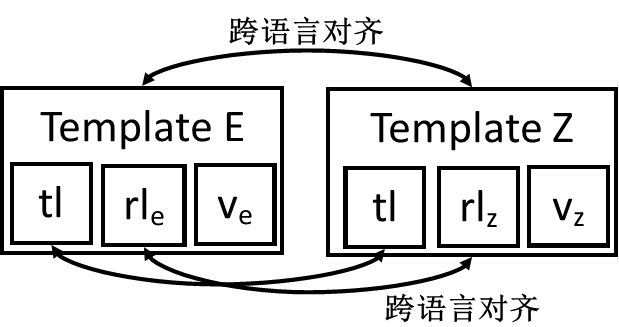
\includegraphics[width=0.8\textwidth]{enwiki-zhwiki-property-crosslinks-1}%为了对齐和上面用的同一张图
%    \caption{基于跨语言实例对齐}
%  \end{subfigure}
%  \vspace{0.01cm}%
%  \begin{subfigure}{0.5\textwidth}
%    \centering
%    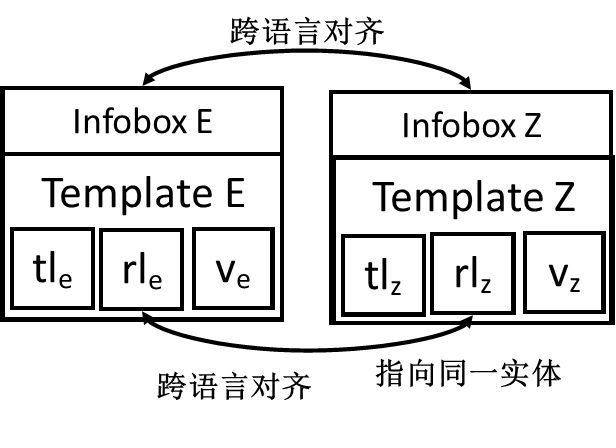
\includegraphics[width=0.8\textwidth]{enwiki-zhwiki-property-crosslinks-3}
%    \caption{基于属性值对齐}
  %\end{subfigure}
  \centering
    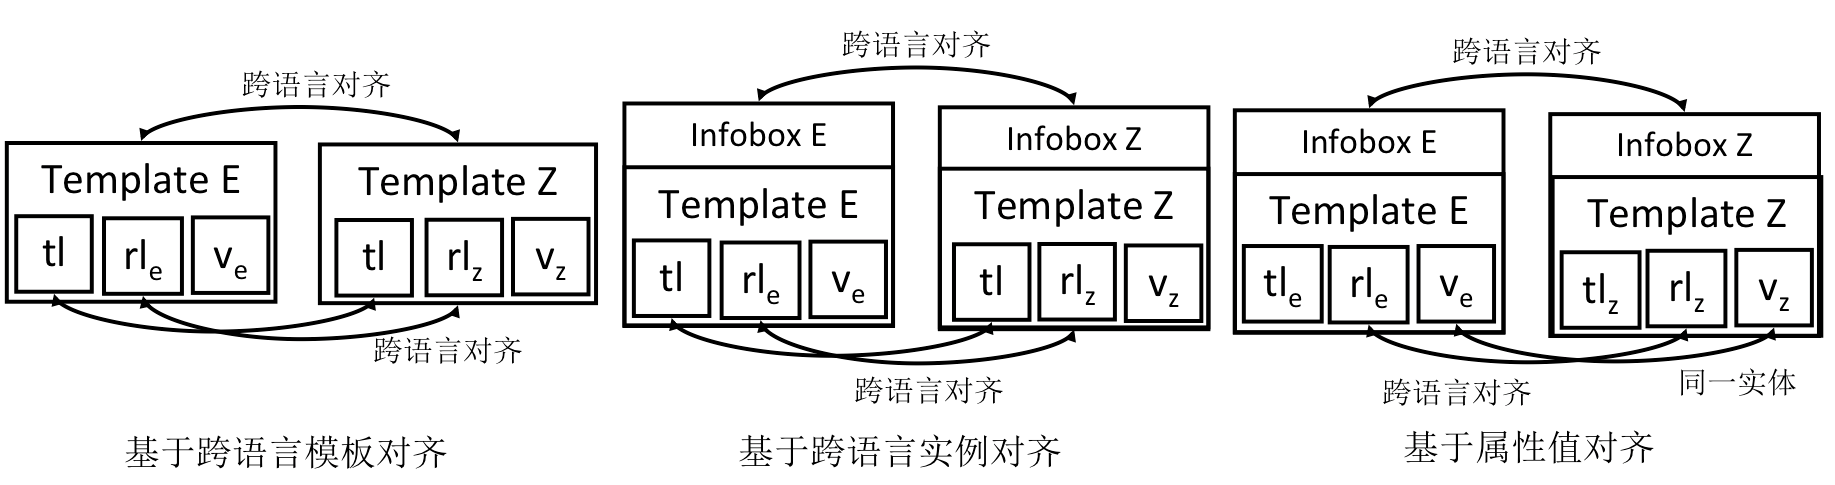
\includegraphics[height=4cm]{cross-lingual-seed}
  \caption{中英文维基属性跨语言抽取说明}
  \label{fig:cross-lingual-seed}
\end{figure}

\begin{enumerate}[1)]
\item  {\heiti 基于跨语言模版对齐:}对于已对齐的跨语言信息框模版$<T_e, T_z>$,找出模板标签一致的中英文显示标签,构成跨语言属性对,即如果$p_e(T_e).tl_e == p_z(T_z).tl_z$,则$<p_e(T_e), p_z(T_z)>$是跨语言链接对;
\item  {\heiti 基于跨语言实例对齐:}对于已对齐的词条$<a_e, a_z>$,抽取其信息框模版$<T_e'(a_e), T_z'(a_z)>$,找出其中模板标签一致的中英文显示标签,构成跨语言属性对,即如果$p_e(T_e').tl_e == p_z(T_z').tl_z$,则$<p_e(T_e'), p_z(T_z')>$是跨语言链接对;
\item  {\heiti 基于属性值对齐:}对于已对齐的词条$<a_e, a_z>$,分析其信息框中的属性-属性值,如果两个中英文属性类型都为对象属性,且属性值指向同一个实体;这两个属性构成跨语言属性对,即如果$a_e(p_e).v is entity \&\& a_z(p_z).v is entity$ 且是跨语言对齐的关系,则$<p_e, p_z>$是属性跨语言链接对。
\end{enumerate}

{\heiti 跨语言种子集合生成},即英文维基与百度百科属性对齐结果,利用前两步的结果作为媒介,两两对齐,获得双语对齐关系。

我们从2016.02版的中文维基与2016.03版的英文维基中获取基于跨语言模版的对齐关系。表\ref{tab:zhwiki-enwiki-cross-lingual}中统计了三种方法分别获得的跨语言属性链接数量和对应举例。最终的跨语言对齐属性种子集合共包含2262个属性,涉及概念领域235个,表\ref{tab:cross-lingual-seed-examples}给出了对齐示例。

\begin{table}[htb]
  \centering
  \caption{中英文维基属性跨语言对齐结果}
  \label{tab:zhwiki-enwiki-cross-lingual}
    \begin{tabular}{ccc}
      \toprule[1.5pt]
      {\heiti 对齐方法} & {\heiti 数量} &  {\heiti 举例} \\\midrule[1pt]
      基于跨语言模板对齐 & 16104 & Editing by  剪辑 Date(s) 日期   \\
      基于跨语言实例对齐 & 124 & 1  memory 记忆体 manufacturer [[制造商]]\\
      基于属性值对齐     & 129 & associated acts 相关团体 num episodes 集数  \\
      总数               & 16357 & -  \\
      \bottomrule[1.5pt]
    \end{tabular}
\end{table}
%
%\begin{table}[htb]
%  \centering
%  \caption{跨语言属性对齐种子集合结果}
%  \label{tab:cross-lingual-seed}
%    \begin{tabular}{ccc}\toprule[1.5pt]
%      {\heiti 对齐数量} & {\heiti 概念数量} \\\midrule[1pt]
%      2262 & 235  \\
%      \bottomrule[1.5pt]
%    \end{tabular}
%\end{table}

\begin{table}[htb]
  \centering
  \caption{跨语言属性对齐种子举例}
  \label{tab:cross-lingual-seed-examples}
    \begin{tabular}{ccc}\toprule[1.5pt]
      {\heiti 概念} & {\heiti 英文属性} &  {\heiti 中文属性} \\\midrule[1pt]
      \multirow{5}{*}{电影}
      & Box office    & 累计票房/全球票房/票房  \\
      & Budget        & 制片成本/预算/电影投资  \\
      & Directed by   & 导演/编剧  \\
      & Distributed by & 出品公司/发行商/发行方/发行公司  \\
      & Release dates & 上映日期/上映/首映日期/上映时间/播放期间  \\
      \midrule[1.0pt]
      \multirow{5}{*}{大学}
      & Active       & 创建时间/建立时间/创办时间/办学时间  \\
      & Affiliations & 主管部门  \\
      & Former names & 老校名  \\
      & Location     & 所属地区/地址/校址/学校地址  \\
      & President    & 院长/董事长/现任校长/现任院长 \\
      \bottomrule[1.5pt]
    \end{tabular}
\end{table}

\subsection{跨语言属性对齐}
\label{sec:cross-lingual-property-matching}
我们将跨语言属性对齐设计成二分类任务,并采用逻辑斯谛回归模型进行训练与预测。

\subsubsection{特征选择}
特征选用三类特征:基于文本特征、基于结构特征、基于分布特征。

{\heiti 基于文本特征} 我们对属性标签和属性值两部分文本分别进行相似度计算。针对语言的差异,我们利用百度翻译API\footnote{\url{http://fanyi.baidu.com/}},获得属性标签中译英、英译中两类翻译结果,与属性值英译中翻译结果。

文本相似度多采用编辑距离(Edit Distance)计算,编辑距离相似度被定义为:
\begin{equation}
ed\_sim(s_1, s_2) = \frac{1}{1+edis(s_1,s_2)}
\end{equation}
\begin{equation}
edis(s_1,s_2)=\frac{edit\_distance(s_1, s_2))}{max(\left| s_1 \right |,\left | s_2 \right |))}
\end{equation}
其中$edit\_distance(s_1, s_2))$表示字符串$s_1$和$s_2$的编辑距离,即由$s_1$变化到$s_2$所需的增、删、改的最小操作数。

标签相似度:对中英文属性的标签进行计算,转换成同语言后,分别进行中文相似度计算与英文相似度计算,取最大值作为特征值。
\begin{equation}
\label{}
sim_{label}(sp_e, sp_z) = max(ed\_sim(label(p_e), label'(p_z)), ed\_sim(label'(p_e), label(p_z)))
\end{equation}
其中$label'$为属性标签对应的翻译字符串。

属性值相似度:属性值是衡量两个属性是否对齐的最直接指标,如果对齐词条下的两个属性含有相同属性值,它们匹配的可能性就很大。根据属性值的内容,我们将其分为三类,分别为文章型、数字型、纯文本型,每一种类型,采用不同的相似度计算策略。

文章型属性值:如果属性值表示一个实体,即其链接到一个词条,认为它是文章型属性。这类属性,对于其“相等”的定义为:如果两个实体是跨语言链接关系,即表征同一实体,则认为属性值相等:
\begin{equation}
Equal(a,a')=\left\{\begin{matrix}
1 \quad  if <a,a'> in \ CL\\
0 \quad  else
\end{matrix}\right.
\end{equation}

文章型属性的相似度计算公式如\ref{equ:article_value_similarity}:

\begin{equation}
\label{equ:article_value_similarity}
sim_{article\_v}(sp_e, sp_z) = \frac{\sum_{a_e\in A(sp_e), a_z \in A(sp_z)} Equal(a_e, a_z)}{min(\left| A(sp_e)\cap CL \right|, \left|A(sp_z) \cap CL) \right|)}
\end{equation}
$A(sp)\cap CL$为含有跨语言链接的词条集合。

数字型属性值:由数字构成的值,比如年龄、日期、电影票房等,被定义为数字型属性值。对于这类属性值,不能直接对比,也不适合用文本相似度计算方法。我们还面临异构百科带来的属性值多样化表达问题:不同百科中,相同词条同一属性的属性值可能由不同形式表示,比如迈克尔·菲尔普斯(Michael Phelps)在英文维基中,身高(Height)为“6 feet 4 inches”,而在百度百科中则表示成193cm。考虑到以上特点,我们用皮尔逊积矩相关系数(Pearson product-moment correlation coefficient)计算数字型属性值的相似度,该系数衡量两个变量的线性相关程度。具体见公式\ref{equ:number_value_similarity}。
\begin{equation}
\label{equ:number_value_similarity}
sim_{number\_v}(sp_e, sp_z) =
\end{equation}

文本型属性值:既不指向实体,又没有数字特征的属性值,被认为是文本型属性值。我们用编辑距离方法计算其相似度\ref{}:
\begin{equation}
\label{equ:literal_value_similarity}
sim_{literal\_v}(sp_e, sp_z) = \frac { \sum _{ { a }_{ e }\in { A }_{ e },{ a }_{ z }\in { A }_{ z } }{ ed\_ sim\left( { a }_{ e }.v,{ a }_{ z }.v \right)  }  }{ \sum _{ { a }_{ e }\in { A }_{ e },{ a }_{ z }\in { A }_{ z } }{ Equal\left( { a }_{ e },{ a }_{ z } \right)  }  }
\end{equation}
其中$a_e, a_z$分别为$a_e(sp_e), a_z(sp_z)$的简写,表示包含属性$sp$的词条;$A_e, A_z$分别为$A_e(sp_e),A_z(sp_z)$的简写,表示使用属性$sp$的所有词条集合。

为了减小计算复杂度并提高准确度,我们将属性值相似度的计算粒度设定为单个文章,即只与对齐文章信息框内的属性值进行比对。

{\heiti 基于结构特征}
当前大部分跨领域的知识库都以在线百科为数据源而建立。百科内部本身就存在着一些语义关系,比如子分类和父分类间的\textit{subClassOf}关系、词条实体与分类之间的\textit{instanceOf}关系。语义信息常被用来抽取特征\cite{wang2014cross},表示实例等在结构上的特点。我们利用百科里现有的语义关系,抽取出两个特征,分别为词条相似度$sim_{article}$与分类相似度$sim_{category}$。文章相似度即计算使用两属性词条的交集(公式\ref{equ:sim-article}),概念相似度即计算两属性领域的相似程度(公式\ ref{equ:sim-category})。我们用标准谷歌距离(Normalized Google Distance,简称NGD)来进行相似度计算。
\begin{equation}
\label{equ:sim-article}
sim_{article}(sp_e, sp_z) = \frac{\max\{\log |A_e|, \log |A_z|\} - \log|A_e \cap A_z|}
{\log |A(sp_e) \cup A(sp_z)| - \min\{\log |A_e|, \log |A_z|\}}
\end{equation}
\begin{equation}
\label{equ:sim-category}
sim_{category}(sp_e, sp_z) = \frac{\max\{\log |Ca_e|, \log |Ca_z|\} - \log|Ca_e \cap Ca_z|}
{\log |Ca(sp_e) \cup Ca(sp_z)| - \min\{\log |Ca_e|, \log |Ca_z|\}}
\end{equation}
其中$A_e, A_z$分别为$A_e(sp_e),A_z(sp_z)$的简写,表示使用属性$sp$的所有词条集合:$Ca_e, Ca_z$分别为$Ca_e(sp_e), Ca_z(sp_z)$的简写,表示属性$sp$相关的分类;

%基于语义的特征表征的是两个
{\heiti 基于分布特征}
是基于假设:\textit{同一属性即使在不同百科中,被使用频率也相近。}我们称之为受欢迎(Popular)程度,该特征的定义为:
\begin{equation}
sim_{popular}(sp_e, sp_z) = abs(\frac{|A(sp_e)|}{|A(C_e)|} - \frac{|A(sp_z)|}{|A(C_z)|})
\end{equation}

\subsubsection{实验结果}

{\heiti 评测标准}
作为标准的二分类模型,我们用准确率(Precision),召回率(Recall),与F1值(F1-Measure)来评测跨语言属性对齐方法。

(1)准确率$Precision$:对齐结果中正确的数量与找到的对齐总数的比值:
\begin{align}
Precision = \frac { \left| A\cap T \right|  }{ \left| A \right|  }
\end{align}

(2)召回率$Recall$:对齐结果中正确的数量与全部已知对齐对数的比值:
\begin{align}
Recall = \frac { \left| A\cap T \right|  }{ \left| T \right|  }
\end{align}

(3)$F1-Measure$:是结合准确率与召回率的总体评价:
\begin{align}
F1-Measure = \frac { 2PR }{ P+R }
\end{align}

我们的训练与测试数据来自\ref{sec:cross-lingual-seed}中抽取的跨语言属性链接种子。取2000个为正例,随机组合取2000个负例,带入逻辑斯谛回归模型。最终结果显示在表\ref{tab:property-matching-result}。
\begin{table}[htb]
  \centering
  \caption{跨语言属性对齐方法评测结果}
  \label{tab:property-matching-result}
    \begin{tabular}{cccc}\toprule[1.5pt]
      {\heiti 方法} & {\heiti 准确率} &  {\heiti 召回率} & {\heiti F1值}  \\ \midrule[1pt]
      跨语言属性对齐 & 83.4\% & 52.6\% & 64.5\% \\
      \bottomrule[1.5pt]
    \end{tabular}
\end{table}

%\begin{table}[htb]
%  \centering
%  \caption{跨语言属性对齐方法结果举例}
%  \label{tab:property-matching-examples}
%    \begin{tabular}{ccc}\toprule[1.5pt]
%      {\heiti 概念} & {\heiti 英文属性} &  {\heiti 中文属性} \\\midrule[1pt]
%      \multirow{5}{*}{电影}
%      & Box office    & 累计票房/全球票房/票房  \\
%      & Budget        & 制片成本/预算/电影投资  \\
%      & Directed by   & 导演/编剧  \\
%      & Distributed by & 出品公司/发行商/发行方/发行公司  \\
%      & Release dates & 上映日期/上映/首映日期/上映时间/播放期间  \\
%      \midrule[1.0pt]
%      \multirow{5}{*}{大学}
%      & Active       & 创建时间/建立时间/创办时间/办学时间  \\
%      & Affiliations & 主管部门  \\
%      & Former names & 老校名  \\
%      & Location     & 所属地区/地址/校址/学校地址  \\
%      & President    & 院长/董事长/现任校长/现任院长 \\
%      \bottomrule[1.5pt]
%    \end{tabular}
%\end{table}
%
%
%此外,对不同特征做出的贡献,我们也在表\ref{tab:feature-compare}中给出了对比:
%
%\begin{table}[htb]
%  \centering
%  \caption{特征组合对结果的影响}
%  \label{tab:feature-compare}
%    \begin{tabular}{cccc}\toprule[1.5pt]
%      {\heiti 特征组合} & {\heiti 准确率} &  {\heiti 召回率} & {\heiti F1值}  \\ \midrule[1pt]
%       $sim_{label}$& 83\%       & 50\% & 1  \\
%       $sim_{label}$+sim_{value} & 83\% & 50\% & 1  \\
%       $sim_{label}$+sim_{value} & 83\% & 50\% & 1  \\
%       $sim_{label}$+sim_{value}+sim_{popular}& 83\% & 50\% & 1  \\
%      \bottomrule[1.5pt]
%    \end{tabular}
%\end{table}


\section{本章小结}
本章主要解决英文维基与百度百科两个异构百科之间的跨语言属性对齐问题。
为了尽可能找到更多属性对齐,我们提出跨语言属性对齐框架,该框架由概念属性生成、同语言属性对齐与相似属性合并、跨语言对齐种子生成以及跨语言属性对齐四部分组成。概念模板针对百度百科没有信息框模板信息的情况,以维基模板为指导抽象出百度百科下的对应概念与属性集合,首先实现概念模板层次的对齐;同语言属性对齐模块给出中文维基与百度百科的对齐策略,获得高准确率的异构百科下的属性对齐关系与属性多表达集合;跨语言对齐种子集合生成模块将中文维基作为媒介,抽取出精准的英文维基与百度百科的中英文属性对齐关系;最终我们基于文本、语义、分布三类特征,训练出跨语言属性对齐二分类模型,作为最终结果。



\chapter{XLore系统与应用接口构建}
\label{cha:xlore-system-api}

\section{本章引论}
当前一些知名的知识库将自己的数据展示或发布出来,DBpedia[地址]提供最新的数据集下载、数据统计记录,甚至开源代码;Probase[地址]给出语义关系的数据集供研究人员使用,如is-a关系,同义词等。

中文知识库中,搜狗、百度等将知识图谱商业化,主要用来优化搜索、推荐实体等,百度用户通过搜索能获得图谱中相关实体的链接,但这些知识图谱只供自家公司商用,并没有开放数据。Zhishi.me作为第一个?科研领域的中文知识库,早期提供实体查询接口与SPARQL查询接口,现数据与网站都久未更新。

我们的中英文跨语言知识库XLORE,基于第三章跨语言知识库的数据,提供了数据展示页面、知识搜索功能、SPARQL查询接口、实例关系可视化、实体链接等多项功能,本章将具体阐述XLORE网站系统的搭建与数据接口的构建。

\section{XLore系统介绍}
XLORE网站系统旨在对外显示我们的数据数量与语义关系,并向用户提供便利的数据接口、清晰的数据展示。其对外网址为http://xlore.org。

截止到目前,XLORE网站提供三类知识展示与两种知识查询方式。

\subsection{XLore知识展示}
图\ref{fig:xlore-home}为XLORE网站首页。截止到2016年3月,我们的跨语言知识库中包含有xxx个概念、xxx个实例、xxx个属性。首页以表格的形式提供了顶层及其下两层的概念层及其统计数据,点击左边“+”按钮可获得子概念样例。除此之外,首页列出了一些实例例子,点击可直接查看相应实例页面。

\begin{figure}[H] 
  \centering
  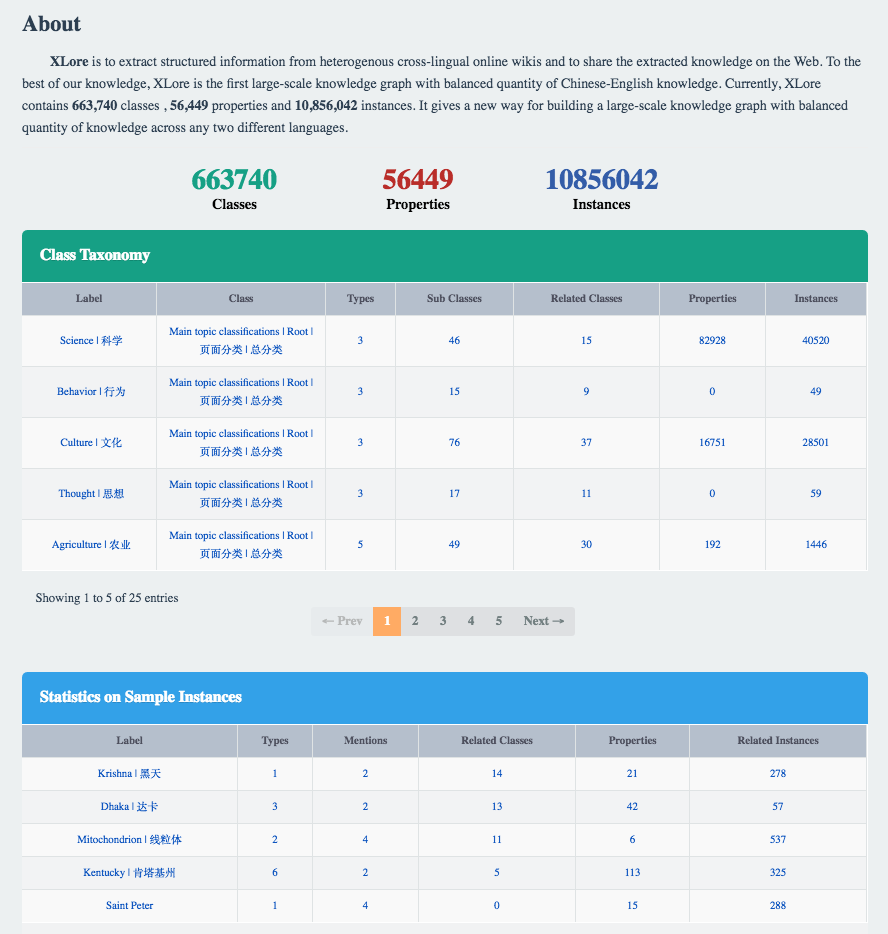
\includegraphics[width=0.8\columnwidth]{xlore-home}
  \caption{XLore网页系统首页}
  \label{fig:xlore-home}
\end{figure}

作为双语知识库,XLORE提供了语言切换功能,同时满足中文用户与外文用户的用户体验。

知识分为三种,分别为概念、属性、实例。概念页面以绿色为主色调,显示了概念中英文标签、父概念、子概念、相关实例等信息。属性页面使用紫色色调,展示了中英文标签、属性类型(Datetype与Objecttype)、相关实例、xx与xx等。

实例页面色调为蓝色,展示了中英文标签、实例图像、所属概念、摘要、信息框(包括中英文信息),URL多种信息。三种页面中,涉及到的双语内容,我们以“中文[英文]”的格式展示每条信息,如果网站语言为英文,则将英文展示在前,格式变为英文[中文]。当涉及到四个百科内容且无法融合,我们利用网页标签分栏的形式分别展示不同百科信息,如图\ref{fig:xlore-page}。

\begin{figure}[H] 
  \centering
  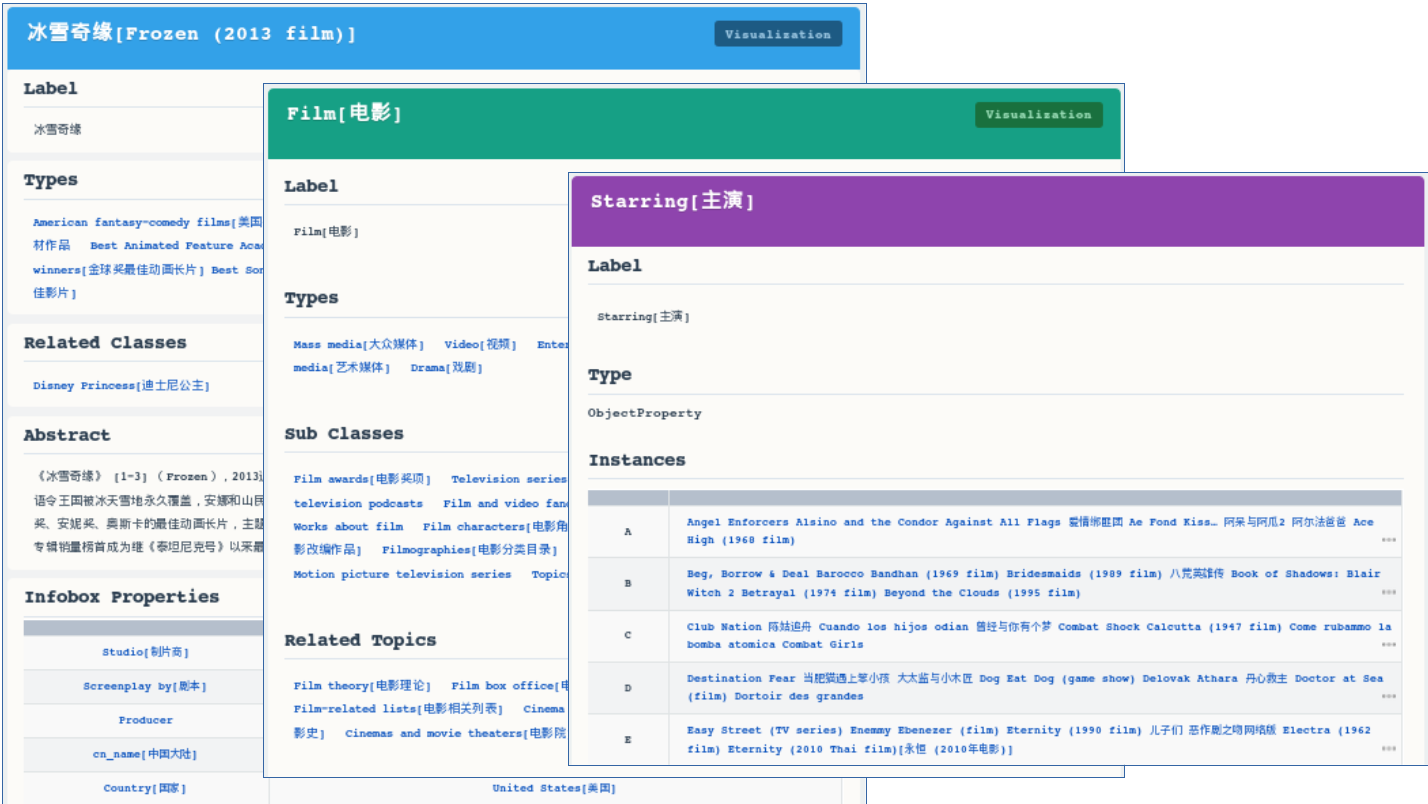
\includegraphics[width=1\columnwidth]{xlore-page}
  \caption{XLore实例、概念、属性页面展示}
  \label{fig:xlore-page}
\end{figure}

\subsection{XLore知识查询}
XLore提供搜索框文本查询与SPARQL语句查询。

搜索框在每个页面上都有,输入要查询的中文或英文字符串,点击“搜索”或按Enter键,即获得模糊查询结果。用户可根据需求选择搜索概念还是实例,或者属性,默认情况下,我们会同时返回三类搜素结果,用户可通过切换标签查看。图\ref{fig:xlore-search-engine}为搜索结果页面展示。

\begin{figure}[H] 
  \centering
  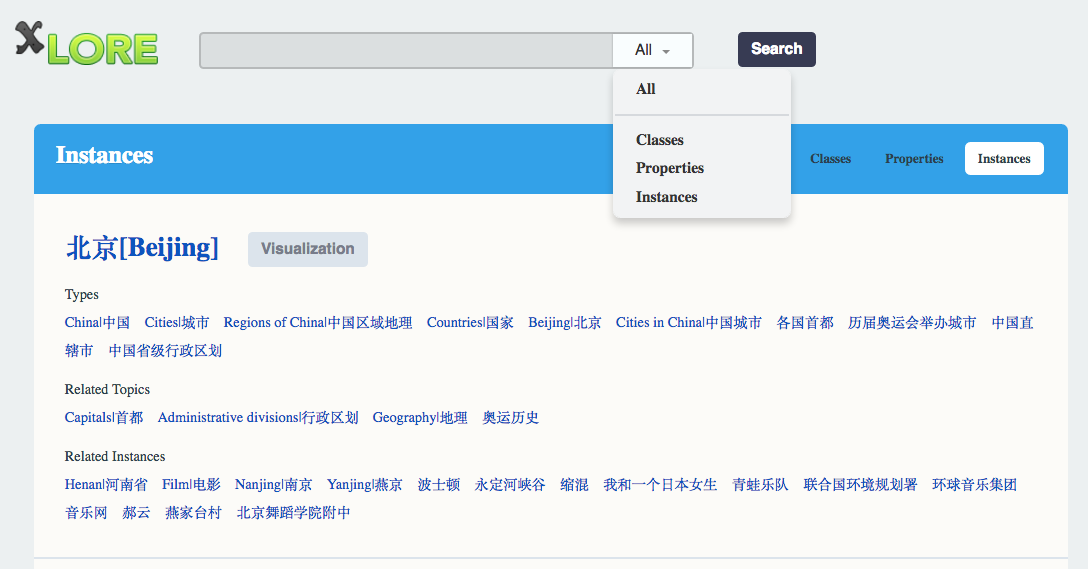
\includegraphics[width=0.9\columnwidth]{xlore-search-engine}
  \caption{XLore文本搜索框与搜索结果展示}
  \label{fig:xlore-search-engine}
\end{figure}

另一方面,对于专业人士,我们提供SPARQL查询页面,如图\ref{fig:xlore-sparql-endpoint}所示,输入正确的sparql语句,返回结果中可看到我们对知识库schema的定义。另外,为了防止sql注入造成的攻击与数据库崩溃,我们采取了xxx的安全措施。

\begin{figure}[H] 
  \centering
  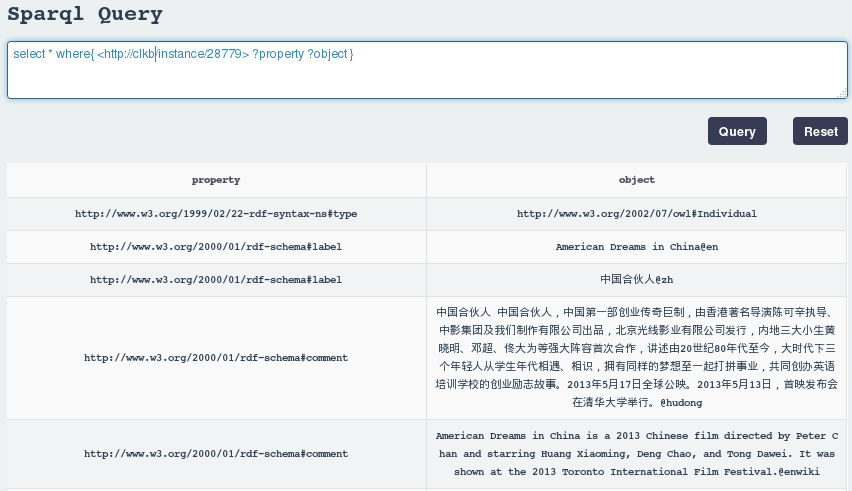
\includegraphics[width=0.9\columnwidth]{xlore-sparql-endpoint}
  \caption{XLore SPARQL 搜索框与搜索结果展示}
  \label{fig:xlore-sparql-endpoint}
\end{figure}

\subsection{XLore系统构建}
图xx为XLORE系统架构图。

xxx语义数据,我们的数据依托于图数据库。当前知名的的图数据库有Neo4J[引用],AllegroGraph[引用],Virtuoso等,鉴于我们的数据是以三元组的形式组织的,更适用于triple-store类型的数据库,因此我们选用商业版Virtuoso[网址](Virtuoso Universal Server)作为存储容器。

Virtuoso是由OpenLink软件公司开发的一个混合型数据库,它既支持传统的RDBMS数据,也支持RDF等其他图类型数据的存储与查询。其商业版本(Virtuoso Universal Server)可支持多CPU处理、多会话访问以及集群网络环境等。商业版Virtuoso是闭源的,但OpenLink公司提供一个名为OpenLink Virtuoso的开源版本[GitHub链接],供使用者编译与尝试。

为了提高搜索效率与召回率,我们对

Web框架采用JSP+Struts2.0搭建,运行在Tomcat7.0 Web服务器上。页面设计基于当前最受欢迎的Bootstrap前段框架。
对于概念与实例,我们基于D3.js可视化库[网址],提供了关系可视化,包括概念-子概念的关系,实例-相关实例的关系。图xx为可视化例子。

\section{XLore实体链接接口}

对同一个实体,外界有不同的称呼,比如演员xx,有昵称aa,bb,再比如电影yy,有名称dd,ee。另一方面,一个名称可能表征不同实体,比如xxxx。给出一个名称,在知识库中找出其对应的真正实体,被称作“实体链接”任务。如果我们能成功抽取出文本中的实体名称,并准确匹配出名称所代表的实体,对于该文本的理解有很大意义。Xxx任务中,xxxx(ji heng老师那个比赛),文章[][][]分别从xx,xxx,xx的数据集中,抽取出实体名称,提出相应的消歧算法,链接到xx知识库中。

XLORE作为一个通用领域的跨语言知识库,也提供了基于实体-名称词典扩展的实体链接接口。

XLORE实体链接接口提供了三种类型的查询:
1.  通用领域的名称查询:给出一个通用领域的名称,返回其在XLORE中最可能指向的一个或几个实体以及实体的中英文信息;
2.  通用领域的文本实体查询:给出一串文本,对文本进行实体名称抽取后,返回名称列表中各名称在XLORE中最可能指向的实体及实体的中英文信息;
3.  学术领域的名称查询:给出一个学术领域的名称,如“机器学习”,返回其在XLORE中学术领域指向的实体以及实体的中英文信息。

该接口框架图如下

具体来说,该接口以中英文名称或文本为输入,经过实体抽取、实体候选生成、实体消歧,确定与名称和上下文最匹配的实体,返回实体列表与中英文实体信息。


\subsection{实体抽取}
通用领域实体抽取使用xxx方法,主要获得xx,xxx,xxx类型的实体。
学术领域实体抽取采用xxx方法,该方法xxxx。

\subsection{实体候选生成}

实体候选从名称-实体词典中,通过名称获取相应的所有实体。其中,中英文名称-实体词典从中英文维基百科、百度百科、互动百科中抽取,选取以下几种元素构成:

1.  各百科的词条标题:百科中的每个词条都描述唯一实体,并维护着这个实体的相关信息。一般来说,词条标题是该实体公认的、最普遍的名称。对于无歧义的标题,记录其完整标题即可。然而,有些标题有多种含义。在百科中,如果一个标题有歧义,百科会通过在标题后加入分类信息来实现消歧,比如百度百科中,苹果(蔷薇科苹果属果实)代表一种水果,苹果(苹果产品公司)代表美国一家高科技公司,这种情况,标题“苹果”为实体“苹果(蔷薇科苹果属果实)”(在XLORE中有对应ID)的一个名称。

2.  各百科的文本内链接:百科词条的文本中,经常会有一些实体名称,以超链接的形式存在,指向该实体对应的词条。这个超链接的锚文本,可以看作是指向实体的同义词或别称,锚文本与实体词条构成一条名称-实体信息。

3.  各百科的消歧页面:如果一个名称可能对应多个实体,百科会为其创建一个歧义页面,供用户按所需选择词条。比如,“苹果”是一个歧义词汇,则歧义页面中会列举“苹果(蔷薇科苹果属果实)”、“苹果产品公司”等词条。维基百科通过“苹果\_(消歧义)”这样的页面[链接地址]展示词条,百度百科则通过为“苹果”父词条[链接地址]创建subview子词条来进行区分,如果一个词条没有歧义,则它的网页地址以id定位;如果一个词条有多种意思,则它的id页面为歧义页面,各子词条网址用subview id定位。消歧页面对于抽取实体的别称也有很大贡献。

4.  维基百科的重定向页面: 维基百科通过不断进行词条整理与更新,对一些陈旧的、非标准词条,或公认的缩写名称、别称等,将其自动定位到同一实体的标准词条页面上。原来的旧名称、缩写等可以看作实体的名称。比如中文维基中,“Microsoft”会被重定向到“微软”页面。

以2016年3月的中英文维基百科、2014年12月的百度百科、互动百科为数据源,我们获得名称-实体关系数量如表 \ref{tab:mention-entity}所示:

\begin{table}[htb]
  \centering
  \caption 名称-实体关系对抽取数量统计
  \label{tab:mention-entity}
  \begin{minipage}[t]{0.8\textwidth} % 如果想在表格中使用脚注,minipage是个不错的办法
    \begin{tabularx}{\linewidth}{l|X|X|X|X|}
      {\heiti } & {\heiti 英文维基} & {\heiti 中文维基} & {\heiti 百度百科} & {\heiti 互动百科} \\\midrule[1pt]
      标题 & 1 & 1 & 1 & 1 \\
      内链接 & 1 & 1 & 1 & 1 \\
      消歧页面 & 1 & 1 & 1 & 1 \\
      重定向页面 & 1 & 1 & 1 & 1 \\
      \bottomrule[1.5pt]
    \end{tabularx}
  \end{minipage}
\end{table}

最终获得中英文名称-实体对应关系总数量为:xxx对。
在抽取过程中,我们对名称-实体的出现频数进行了记录,用于之后的排歧工作,将会在xxx章详细说明。以”名称\\t实体知识库uri\\t该对出现频数”为格式存储数据,并以名称为索引,将数据导入到MySQL数据库中。

\subsection{实体消歧方法}
对于通用领域的名称查询,因为没有任何上下文信息,我们只能直接以频数从高到低排序,返回受认可的一个或多个实体信息。

对于通用领域的文本查询,我们根据上下文,为每个名称返回最相关的实体。具体来说:
\begin{itemize}
\item 1.  计算文本相关度:认为自身信息与上下文有关的实体更相关,提取实体上下文,与实体的摘要进行cosine相似度计算。
\item 2.  计算语义相关度:认为与文中其他实体有语义关系的实体更相关:提取根据文中其他实体,找出相关概念,xxxx。
\item 3.  取两个相关度的最大值。
\end{itemize}

对于学术领域的名称查询,我们利用知识库特有的领域限制,将实体的查找限制在相关概念下。

\subsection{实体链接接口的应用}
该实体链接接口的学术领域名称查找功能,应用在Aimer学术搜索系统[引用]的学术知识展示模块上,如图xx所示:用户在搜索学术领域词汇时,右边会显示该词汇对应的学术实体信息,及其相关上下文概念。

\section{本章小结}
本章对XLORE系统进行了详尽的介绍。为了进一步了解数据情况,我们搭建了网站展示XLORE知识,将数据直观地展现出来。同时,为了提高知识库的可用性,开发了实体链接接口,提供通用领域与指定领域的语义信息,也为下一步更精确的实体链接工作,做好铺垫。








\chapter{总结与展望}
\label{cha:conclusion}
本章对本文涉及的工作内容进行了概括与总结,并从属性对齐、知识库构建与应用角度出发,提出待改进之处。

\section{现有工作总结}
本文对维基百科与百度百科的信息框模板与属性进行了深入的研究,涉及到跨语言与跨百科两部分问题。通过对数据细致入微的观察,本文通过模式匹配、相似度计算等方法,生成维基百科与百度百科中的概念与对应属性集合,并计算出异构百科中的跨语言信息框属性对齐关系。同时,将属性对齐结果应用于跨语言知识库XLore的构建中。

首先,在同百科跨语言研究上,我们对维基百科的信息框编辑机制进行了详细的分析,发掘出信息框模板组织方式与属性的定义模式,并基于此做了两项工作:1. 维基百科显示标签的抽取;2. 根据信息框模板提供概念,并生成概念属性。最终获得的结果覆盖90\%以上词条,为后续异构百科的属性分析提供了重要信息。

其次,在异构百科跨语言研究过程中,我们面临百度百科中属性的歧义与多表示问题。从模板得到启发,我们为以维基模板概念为指导,为百度属性划分领域,在领域范围内对齐属性,避免属性多义问题。另在同语言百科对齐同时查找属性同义表达。以中文维基为桥梁,首先获得一批准确的英文维基与百度百科的对齐关系,以此为种子集合,提出基于文本、语义、分布三类特征,训练二分类模型,实现异构百科下的跨语言链接。

属性的分析结果主要应用于跨语言知识库XLore。该知识库基于中英文维基百科、百度百科、互动百科四个数据源构建,抽取概念、属性、实例,使用跨语言链接融合中英文知识。最终结构化数据转换为标准的RDF三元组。基于该知识库数据,我们建立了XLore.org展示系统,提供知识的可视化与查询。同时,从知识库应用角度,开发了实体链接接口,支持通用领域与学术领域的实体识别与实体链接,返回相关语义信息。该接口应用到学术术语词汇查询、新闻文本分析等领域上。

总体来说,本文的重点在概念属性分析上,并辅助跨语言知识库的构建,该工作对于知识库Schema定义、中英文知识平衡等有着十分积极的意义。此外,本文所提供的维基数据的分析、跨语言知识库建立的流程,对于从结构化数据中构建知识库有很大借鉴意义。

\section{未来工作展望}
在信息框属性的分析因属性粒度小特征少,数据不归整等原因,是一项繁杂的工作。通常来说,分辨属性的最佳特征为属性值,但值文本的复杂性增加了特征提取难度与特征准确性,因此还需要其他特征的辅助,文章、模板、领域等等元素可以作为提取特征的候选,不过在本文工作中并未被充分利用。此外,跨语言对齐受翻译正确率、有限的已知跨语言信息等因素的限制,也需要考虑更独立的方法。

归结起来,本文在信息框属性方面,提出以下几个待提高点:
\begin{enumerate}[1)]
\item {\heiti 相似属性合并:} 属性存在多表示问题,我们提出寻找相似属性的任务来提高被处理属性的召回率。为了减小对后期跨语言对齐的影响,我们舍弃了召回率,保留了基于同语言对齐而提取出的更为精准的属性多表现形式。然而,同语言相似属性的查找依然是属性对齐过程中一个亟待解决的问题。如何通过同语言间的关系,找出更多、更准确的属性表现形式,是我们需要继续研究的工作。
\item {\heiti 抽取更多跨语言属性关系:} 基于维基百科开展的属性对齐研究有很多,大部分是对属性值进行细致地处理后,通过值对齐进而得到属性对齐关系。本文对属性值的分析还不到位,比如属性类别还可以进一步划分出日期、列表等类型,文本属性值还需要进行清理。
\item {\heiti 获取更多跨语言信息:} 跨语言属性关系与特征的抽取都基于跨语言词条,维基百科的语言链接数量有限,会成为属性对齐分析的瓶颈。此外,跨语言信息对构建跨语言知识库也很重要。如何扩展跨语言链接集合,是很有意义的一项研究任务。使用词条与属性链接相互增加迭代的方式,同步扩展两者的跨语言对齐关系,也有必要一试。
\item {\heiti 属性特征提取:} 本文主要从文本、语义等方面提取特征,事实上,结构信息、属性关联度等都可能有一定帮助,充分利用百科结构化信息,有利于我们标识属性,生成更多跨语言链接。
\end{enumerate}

在知识库构建方面,本文所涉及的跨语言知识库XLore融合了四个百科的数据,在对齐数量、数据正确性方面都还有待提高,许多研究点如分类体系的形成、信息框填充、百科缺失链接处理等都可进行深入思考。

知识库的质量与其可用性密切相关,在应用方面,如何广泛、有效利用知识库也值得深究。辅助优化搜索、提供关联信息等都是可以尝试的应用。此外我们希望,涵盖了通用领域知识的XLore,也可以在特定领域中大显身手,面向学术领域的实体链接,即为一个尝试。具体来说,给定一个概念,能在知识库中直接划分出该领域的相关概念、实例、属性,形成领域知识,这就能很好地服务于限定领域的应用。

对于目前已存在的实体链接应用,本文提供了基础解决方案与框架,然而这条路还很长,我们还需要从识别实体文本、精确消歧、解决无信息实体,甚至提高查询响应度等方面,提高接口的可用性。

本章提出了工作需要进行的改进以及可能进行的突破,这些是我们未来工作的方向。为打造一个高质量、实用的跨语言知识库,我们依然要不懈努力。



%%% 其它部分
\backmatter

% 本科生要这几个索引,研究生不要。选择性留下。
\makeatletter
\ifthu@bachelor
  % 插图索引
  \listoffigures
  % 表格索引
  \listoftables
  % 公式索引
  %\listofequations
\fi
\makeatother


% 参考文献
% 注意至少需要引用一篇参考文献,否则下面两行可能引起编译错误。
% 如果不需要参考文献,请将下面两行删除或注释掉。
\bibliographystyle{thuthesis}
\bibliography{ref/refs}

% 致谢
% 如果使用声明扫描页,将可选参数指定为扫描后的 PDF 文件名,例如:
% \begin{ack}[scan-statement.pdf]
\begin{acknowledgement}
  由衷感谢导师李涓子教授在我本科毕业时对我抛出橄榄枝,让我有机会在清华大学继续深造,李老师在研究生期间对我的悉心指导与热心帮助,我将铭记于心, 她的言传身教,令我终生受益。

  真诚感谢张鹏老师在技术上给我的指导,在项目期间对我的包容,他的教导,会成为将来工作岗位上,我的指路明灯。

  在此致谢知识工程实验室的小伙伴们对我学习工作上的帮助与支持,让我能收获知识,完成学业。他们带给我的欢声笑语,将会成为我难忘的回忆。

  最后向我的父母以及其他家人致谢,因为他们的支持、呵护与陪伴,我才能保持一颗单纯的心,毫无顾忌,一心向学,一次次超越自我,战胜困难。希望我的顺利毕业,能回应他们望女成凤的期望之心。

~\\

  特此致谢国家自然科学基金委员会与法国国家科研署双边合作协议(61261130588)、国家重点基础研究发展计划(2014CB340504)、清华大学自主科研项目(20131089256)、国家科技支撑计划(2014BAK04B00)和THU-NUS 下一代搜索联合研究中心项目资助

\end{acknowledgement}


% 附录

% 个人简历
\begin{resume}

  \resumeitem{个人简历}

  1991 年 09 月 27 日出生于河北省廊坊市大厂回族自治县。

  2009 年 9 月考入北京邮电大学软件学院攻读软件工程专业,于 2013 年 7 月本科毕业并获得工学学士学位。 

  2013 年 9 月作为免推研究生,进入清华大学计算机科学与技术系,攻读计算机技术专业硕士至今,在知识工程实验室工作。

  \researchitem{发表的学术论文} % 发表的和录用的合在一起

  % 1. 已经刊载的学术论文(本人是第一作者,或者导师为第一作者本人是第二作者)
  \begin{publications}
    \item Li M., Shi Y., Wang Z. and Liu Y.. Building a Large-Scale Cross-Lingual Knowledge Base from Heterogeneous Online Wikis. Natural Language Processing and Chinese Computing. Springer International Publishing, 2015, 413-420.
    \item Wang Z., Li J., Li S., Li M., Tang J., Zhang K., and Zhang K.. Cross-lingual Knowledge Validation Based Taxonomy Derivation from Heterogeneous Online Wikis. AAAI'14. pp. 180-186.
    \item Wang Z., Li J., Wang Z., Li S., Li M. et al. Xlore: A large-scale english-chinese bilingual knowledge graph. In Proceedings of the 2013th International Conference on Posters \& Demonstrations Track-Volume 1035 (pp. 121-124). CEUR-WS. org.
  \end{publications}

  % 2. 尚未刊载,但已经接到正式录用函的学术论文(本人为第一作者,或者
  %    导师为第一作者本人是第二作者)。
  %\begin{publications}[before=\publicationskip,after=\publicationskip]
  %  \item Yang Y, Ren T L, Zhu Y P, et al. PMUTs for handwriting recognition. In
  %    press. (已被 Integrated Ferroelectrics 录用. SCI 源刊.)
  %\end{publications}

  % 3. 其他学术论文。可列出除上述两种情况以外的其他学术论文,但必须是
  %    已经刊载或者收到正式录用函的论文。
  %\begin{publications}
  %  \item Wu X M, Yang Y, Cai J, et al. Measurements of ferroelectric MEMS
  %    microphones. Integrated Ferroelectrics, 2005, 69:417-429. (SCI 收录, 检索号
  %    :896KM)
  %  \item 贾泽, 杨轶, 陈兢, 等. 用于压电和电容微麦克风的体硅腐蚀相关研究. 压电与声
  %    光, 2006, 28(1):117-119. (EI 收录, 检索号:06129773469)
  %  \item 伍晓明, 杨轶, 张宁欣, 等. 基于MEMS技术的集成铁电硅微麦克风. 中国集成电路,
  %    2003, 53:59-61.
  %\end{publications}

  \researchitem{研究成果} % 有就写,没有就删除
  \begin{achievements}
    \item 李涓子,王志刚,李双婕,李明洋,唐杰. 跨语言本体构建方法及装置: 中国, CN103336852A. 2013.10.02
  \end{achievements}

\end{resume}

\end{document}
